%%%%%%%%%%%%%%%%%%%%%%%%%%%%%%%%%%%%%%%%%%%%%%%%%%%%%%%%%%%%
\documentclass[a4paper,11pt,oneside]{article}
\usepackage[a4paper,vmargin={1.5cm,1.5cm},width=16cm]{geometry}
\usepackage[style=verbose-inote,doi=false,sortcites=true,block=space,backend=bibtex]{biblatex}
\usepackage[utf8]{inputenc}
\usepackage{textcomp}
\usepackage[spanish]{babel}
\usepackage{microtype}
\usepackage{lmodern}
\usepackage{graphicx}
\usepackage{fancyhdr}
\usepackage{booktabs}
\usepackage{eurosym}
\usepackage{mathptmx}
\usepackage[T1]{fontenc}
\usepackage{hyperref}
%% Added to help mimic structure.
\usepackage[many]{tcolorbox}
\usepackage{soul}
\usepackage{color}
\usepackage{lastpage}
%\usepackage[skins]{tcolorbox}
%%%%%%%%%%%%%%%%%%%%%%%%%%%%%%%%%%%%%%%%%%%%%%%%%%%%%%%%%%%%
%% HEADERS
%\setlength{\headheight}{1cm}
%\setlength{\headsep}{0.5cm}
%\pagestyle{fancyplain}
%\fancyhf{}
%\lhead{\fancyplain{}{\sc Memoria científico técnica de proyectos coordinados}}
%\rhead{\fancyplain{}{\sc Parte A}}
%\cfoot{\thepage}
%\renewcommand{\headrulewidth}{0pt} % remove lines
%\renewcommand{\footrulewidth}{0pt}


%%% HEADER
\setlength{\headheight}{1cm}
%\setlength{\headwidth}{20cm}
\setlength{\headsep}{0.5cm}
\pagestyle{fancyplain}
\fancyheadoffset[HR,HL]{2cm}
\fancyhf{}
\lhead{\raisebox{-0.4\height}{
\includegraphics[height=0.9cm,keepaspectratio=true]{img/miniLogo}}}
\rhead{\fancyplain{}{\fontsize{10}{12} \selectfont \textbf{\underline{Memoria científico técnica de proyectos coordinados}}}}
\cfoot{\thepage\, / parte A}
\renewcommand{\headrulewidth}{0pt} % remove lines
\renewcommand{\footrulewidth}{0pt}
%%%%%%%%%%%%%%%%%%%%%%%%%%%%%%%%%%%%%%%%%%%%%%%%%%%%%%%%%%%%
%% Hack to make math formulas bold in section titles
\makeatletter
\DeclareRobustCommand*{\bfseries}{%
  \not@math@alphabet\bfseries\mathbf
  \fontseries\bfdefault\selectfont
  \boldmath
}
\makeatother

%%%%%%%%%%%%%%%%%%%%%%%%%%%%%%%%%%%%%%%%%%%%%%%%%%%%%%%%%%%%
\def\thesection{\bf \textsf{\Alph{section}}}

%\nobibliography{biblio}
%\bibliographystyle{JHEP}

\bibliography{biblio}


%%%%%%%%%%%%%%%%%%%%%%%%%%%%%%%%%%%%%%%%%%%%%%%%%%%%%%%%%%%%
\begin{document}

%% Some useful definitions
% BB
\newcommand{\bb}{\ensuremath{\beta\beta}}
% BB0NU
\newcommand{\bbonu}{\ensuremath{\beta\beta0\nu}}
% BB2NU
\newcommand{\bbtnu}{\ensuremath{\beta\beta2\nu}}
% NME
\newcommand{\Monu}{\ensuremath{\Big|M_{0\nu}\Big|}}
\newcommand{\Mtnu}{\ensuremath{\Big|M_{2\nu}\Big|}}
% PHASE-SPACE FACTOR
\newcommand{\Gonu}{\ensuremath{G_{0\nu}(\Qbb, Z)}}
\newcommand{\Gtnu}{\ensuremath{G_{2\nu}(\Qbb, Z)}}

% mbb
\newcommand{\mbb}{\ensuremath{m_{\beta\beta}}}
\newcommand{\kgy}{\ensuremath{\rm kg \cdot y}}
\newcommand{\ckky}{\ensuremath{\rm counts/(keV \cdot kg \cdot yr)}}
\newcommand{\mbba}{\ensuremath{m_{\beta\beta}^a}}
\newcommand{\mbbb}{\ensuremath{m_{\beta\beta}^b}}
\newcommand{\mbbt}{\ensuremath{m_{\beta\beta}^t}}
\newcommand{\nbb}{\ensuremath{N_{\beta\beta^{0\nu}}}}

% Qbb
\newcommand{\Qbb}{\ensuremath{Q_{\beta\beta}}}

% Tonu
\newcommand{\Tonu}{\ensuremath{T_{1/2}^{0\nu}}}

% Tonu
\newcommand{\Ttnu}{\ensuremath{T_{1/2}^{2\nu}}}

% Xe-136
\newcommand{\Xe}{\ensuremath{^{136}}Xe}

% 2S
\newcommand{\TwoS}{\ensuremath{^{2}S_{1/2}}}

\newcommand{\TwoP}{\ensuremath{^{2}P_{1/2}}}

\newcommand{\TwoD}{\ensuremath{^{2}D_{3/2}}}


% Xe-136
\newcommand{\CS}{\ensuremath{^{137}}Cs}

% Xe-136
\newcommand{\NA}{\ensuremath{^{22}}Na}


% Bi-214
\newcommand{\Bi}{\ensuremath{^{214}}Bi}

% Tl-208
\newcommand{\Tl}{\ensuremath{^{208}}Tl}

% Pb-208
\newcommand{\Pb}{\ensuremath{^{208}}Pb}
% Pb-208
\newcommand{\PBD}{\ensuremath{^{210}}Pb}

% Po-214
\newcommand{\Po}{\ensuremath{^{214}}Po}

% bru
\newcommand{\bru}{cts/(keV$\cdot$kg$\cdot$y)}
\newcommand{\HPXE}{\sc{HPXe}\rm}
\newcommand{\BATA}{\sc{BaTa}\rm}

% Saltos de carro en tablas
\newcommand{\minitab}[2][l]{\begin{tabular}{#1}#2\end{tabular}}

\newcommand{\thedraft}{0.1.1}% version for referees

\newcommand{\MO}{\ensuremath{{}^{100}{\rm Mo}}}
\newcommand{\SE}{\ensuremath{{}^{82}{\rm Se}}}
\newcommand{\ZR}{\ensuremath{{}^{96}{\rm Zr}}}
\newcommand{\KR}{\ensuremath{{}^{82}{\rm Kr}}}
\newcommand{\ND}{\ensuremath{{}^{150}{\rm Nd}}}
\newcommand{\XE}{\ensuremath{{}^{136}\rm Xe}}
\newcommand{\GE}{\ensuremath{{}^{76}\rm Ge}}
\newcommand{\GES}{\ensuremath{{}^{68}\rm Ge}}
\newcommand{\TE}{\ensuremath{{}^{128}\rm Te}}
\newcommand{\TEX}{\ensuremath{{}^{130}\rm Te}}
\newcommand{\TL}{\ensuremath{{}^{208}\rm{Tl}}}
\newcommand{\CA}{\ensuremath{{}^{48}\rm Ca}}
\newcommand{\CO}{\ensuremath{{}^{60}\rm Co}}
\newcommand{\PO}{\ensuremath{{}^{214\rm Po}}}
\newcommand{\U}{\ensuremath{{}^{235}\rm U}}
\newcommand{\CT}{\ensuremath{{}^{10}\rm C}}
\newcommand{\BE}{\ensuremath{{}^{11}\rm Be}}
\newcommand{\BO}{\ensuremath{{}^{8}\rm Be}}
\newcommand{\UDTO}{\ensuremath{{}^{238}\rm U}}
\newcommand{\CD}{\ensuremath{^{116}{\rm Cd}}}
\newcommand{\THO}{\ensuremath{{}^{232}{\rm Th}}}
\newcommand{\BI}{\ensuremath{{}^{214}}Bi}


%% Heading
\begin{tcolorbox}[colback=white,arc=0pt,outer arc=0pt,colframe=black,boxrule=0.6pt]
\begin{center}
Convocatorias 2015\\ 
Proyectos Excelencia y Proyectos RETOS \\ 
Dirección General de Investigación Científica y Técnica \\
Subdirección General de Proyectos de Investigación
\end{center} 
\end{tcolorbox}

\begin{tcolorbox}[colback=yellow,arc=0pt,outer arc=0pt,colframe=black,boxrule=0.6pt,left=0mm,right=0mm]
  \begin{center}
    AVISO IMPORTANTE\\
  \end{center}
    En virtud del art\'iculo 11 de la convocatoria \ul{\textbf{NO SE ACEPTAR\'AN NI SER\'AN SUBSABABLES MEMORIAS CIENT\'IFICO-T\'ECNICAS}} que no se presenten en este formato.
     \\
    \textbf{La parte C no podrá exceder 25 p\'aginas.}
    \\
    \\
    \textbf{Lea detenidamente las instrucciones para rellenar correctamente esta memoria disponibles en la web de la convocatoria .}
    \\
  %\end{center}
\end{tcolorbox}
\vspace{3pt}
\begin{tcolorbox}[colback=yellow,arc=0pt,outer arc=0pt,colframe=black,boxrule=0.6pt,left=0mm]
  \noindent\textbf{Parte A: RESUMEN DE LA PROPUESTA/SUMMARY OF THE PROPOSAL}
  %\section{RESUMEN DE LA PROPUESTA/SUMMARY OF THE PROPOSAL}
\end{tcolorbox}

%%%%%%%%%%%%%%%%%%%%%%%%%%%%%%%%%%%%%%%%%%%%%%%%%%%%%%%%%%%%%%%%%%%%%%%%%%%%%

%\section{RESUMEN DE LA PROPUESTA/SUMMARY OF THE PROPOSAL}

%%%%%%%%%%%%%%%%%%%%%%%%%%%%%%%%%%%%%%%%%%%%%%%%%%%%%%%%%%%%%%%%%%%%%%%%%%%%%

%\subsection{DATOS DEL PROYECTO COORDINADO}
\noindent\textbf{A.1. DATOS DEL PROYECTO COORDINADO}
\vspace{6pt}

\noindent\textbf{INVESTIGADOR COORDINADOR PRINCIPAL 1:} (Nombre y apellidos)

\noindent José Díaz Medina.
\vspace{6pt}

\noindent\textbf{INVESTIGADOR COORDINADOR PRINCIPAL 2:} (Nombre y apellidos)

\noindent 
\vspace{6pt}

\noindent\textbf{TÍTULO GENERAL DEL PROYECTO COORDINADO:} Desarrollo de un nuevo tipo de aparato PET basado en Xenón Líquido.
\vspace{6pt}

\noindent\textbf{ACRÓNIMO DEL PROYECTO COORDINADO:} PETALO.


\noindent\textbf{RESUMEN DEL PROYECTO COORDINADO} 
{\color{blue}{M\'aximo 3500 caracteres (incluyendo espacios en blanco):}}
\vspace{12pt}

Este proyecto propone una prueba de concepto para un nuevo tipo de aparato PET, denominado PETALO (PET with TOF Applications based in Liquid XenOn). El material activo es xenón líquido leído por fotomultiplicadores de silicio (SiPM). El elemento básico de PETALO es la celda centelleadora de xenón líquido (LXSC), de dimensiones $5\times 5 \times 5$~cm$^3$, optimizada para maximizar el número de gammas que interacciones en la celda y minimizar el pile-up. La configuración con mayor rendimiento de la LXSC instrumenta sus seis caras internas con matrices de 8$\times$8 SiPM de $6 \times 6$~mm$^2$~de superficie (denominamos esta configuración LXSC6). La configuración más económica, que sin embargo mantiene una excelente resolución tanto en energía como en posición, instrumenta sólo la cara de entrada y de salida (relativa a la dirección de los fotones incidentes) y se denomina LXSC2.

El xenón es un gas noble, que centellea en respuesta a la radiación. La señal de centelleo del xenón líquido es muy rápida (2.2 ns) y muy intensa (37,000 fotones por gama de 511 keV). La combinación de ambas características hace posible utilizar el xenón líquido para construir un PET de gran resolución en energía (alrededor del 5\% FWHM, a comparar con el 20\% típico de los PET convencionales modernos) {\em y gran resolución temporal}, lo que permite su aplicación como PET-TOF. La aplicación de tiempo de vuelo para reducir los errores de reconstrucción de imagen en PET, conocida desde el albor de la tecnología ha resurgido con fuerza en los últimos años, en los que se han construido modelos comerciales con resoluciones temporales entre 400 y 600 ps que mejoran considerablemente la resolución de los PET convencionales. PETALO aspira a una resolución temporal en el rango de los 200-250 ps, lo que supondría un salto cuantitativo en la tecnología.

Además de las ventajas anteriores, PETALO se diseña desde el principio como un detector compatible con Resonancia Magnética Nuclear (RMN) y por tanto capaz de operar en combinación con este tecnología.

Por último, dado el bajo coste del xenón comparado con los centelleadores utilizados en los sistemas PET modernos (tales como el LSO) y el uso de la moderna tecnología de SiPMs, cuyo coste ha disminuido exponencialmente en los últimos años, la tecnología propuesta por PETALO podría resultar en un sistema lo bastante económico como para construir aparatos de gran tamaño (PET de cuerpo completo). 

Este proyecto coordina tres grupos cuya experiencia combinada permiten la construcción y puesta a punto de un demostrador de PETALO basado en cuatro LXSC2, llamado P4. El subproyecto DET (IFIC) está a cargo de la construcción del detector, aplicando la tecnología desarrollada en el IFIC en el contexto del experimento NEXT. También desarrollará la simulación y el entorno de software para la operación del detector y se ocupará del estudio de su capacidad como PET-TOF. El subproyecto ASIC (I3M/UPV) está a cargo del desarrollo de la electrónica para operar P4 así como del desarrollo de un ASIC, denominado APE (Asic for PEtalo) específico para esta tecnología. El subproyecto IMG (GIBI239/LaFe) está a cargo del análisis de imagen, la operación y certificación de P4 como instrumento compatible con RMN. 




 
\vspace{12pt}

\noindent\textbf{PALABRAS CLAVE DEL PROYECTO COORDINADO:} PET, xenón líquido, TOF, Resonancia magnética nuclear, SiPM, centelleo, alta resolución.

\vspace{12pt}

\noindent\textbf{TITLE OF THE COORDINATED PROJECT:} Development of a new PET apparatus based in Liquid Xenon 
\vspace{6pt}

\noindent\textbf{ACRONYM OF THE COORDINATED PROJECT:} PETALO.
\vspace{6pt}

\noindent\textbf{SUMMARY OF THE COORDINATED PROJECT} 
\vspace{6pt}

This project proposes a proof-of-concept for a new type of PET apparatus, called
PETALO (PET with TOF Applications based in Liquid XenOn). The active target is liquid xenon (LXe), read by silicon photomultipliers (SiPMs). The basic element of PETALO is the Liquid Xenon Scintillating Cell (LXSC). Its dimensions are $5\times 5 \times 5$~cm$^3$, optimised to maximise the number of gammas that interact in the cell and to minimise pileup. The best performance is obtained for a configuration where all the six faces are instrumented with matrices of  8$\times$8 SiPMs, each of $6 \times 6$~mm$^2$~area (LXSC6). The most economical configuration (LXSC2) instruments only the entry and exit faces (relative to the incoming gammas) but still displays an excellent performance. 

Xenon is a noble gas which scintillates as response to the ionising radiation. The scintillation is very fast (2.2 ns) and very intense (37,000 photons per 511 keV gamma). The combination of both features results in the possibility of building a PET of excellent resolution (better than 5\% FWHM, to be compared with 20\% typical of commercial devices) {\em and excellent time resolution}. This, in turn, makes it possible the application of PETALO as PET-TOF. The use of time of flight to reduce imaging errors is known since the beginning of the technology and the last few years have witnessed a rekindled interest in the technique, including the introduction in the market of a commercial model of 600 ps CRT (Coincidence Resolution Time). Other recent devices feature improved CRT near 400 ps. PETALO could achieve CRTs in the rango of 200-250 ps, thus representing a break-through in the technology.  

In addition of the above advantages, PETALO will be designed from the very beginning as a detector compatible with Nuclear Magnetic Resonance (NMR), thus capable to operate in combination with this technology. 

Last but not least, given the low cost of xenon compared with that of conventional scintillators such as LSO, and the application of the modern SiPM technology (the costs of SiPMs has decreased dramatically over the last few years while their performance has continuously improved), it appears possible that PETALO could result in a low-cost system, suited for a full boy PET.

This projects coordinates three groups whose combined experience permits the construction and commissioning of a demonstrator of PETALO based in 4 LXSC2, called P4. The DET subproject (IFIC) is in charge of the construction and of the detector, transferring to this very applied problem the technology developed in the context of a basic science enterprise, a neutrinoless double beta decay experiment called NEXT. The ASIC subproject (I3M/UPV) is in charge of the development of the electronics to operate P4 as well as of the development of an ASIC optimised for the technology, called APE (Asic for PEtalo). The subproject IMG 
(GIBI239/LaFe) is in charge of image analysis, operation and certification of P4 as a NMR compatible device and the study of its capabilities as a TOF device. 
 





 \vspace{12pt}

\noindent\textbf{KEYWORDS OF THE COORDINATED PROJECT:} PET, scintillation, liquid xenon, SiPMs, high resolution, TOF, Nuclear magnetic resonance.  

 \vspace{12pt}
%\newpage

%%%%%%%%%%%%%%%%%%%%%%%%%%%%%%%%%%%%%%%%%%%%%%%%%%%%%%%%%%%%%%%%%%%%%%%%%%%%%

\noindent\textbf{A.2. DATOS DE LOS SUBPROYECTOS/ DATA OF SUBPROJECTS }
 \vspace{12pt}
 
\noindent\textbf{SUBPROYECTO 1 / SUBPROJECT 1} (el investigador o investigadores principales son los coordinadores del proyecto coordinado)

\vspace{6pt}
\noindent\textbf{TÍTULO / TITLE :} PETALO-DETECTOR (PETALO-DET)

 \vspace{12pt}
 
\noindent\textbf{SUBPROYECTO 2 / SUBPROJECT 2}
\vspace{6pt}

\noindent\textbf{INVESTIGADOR PRINCIPAL 1 / PRINCIPAL RESEARCHER 1 } (nombre y apellidos)

\vspace{6pt}
\noindent Vicente Herrero Bosch

\vspace{12pt}
\noindent\textbf{INVESTIGADOR PRINCIPAL 2 / PRINCIPAL RESEARCHER 2} (nombre y apellidos)

\vspace{6pt}
Rafael Gadea Gironés


\vspace{6pt}
\noindent\textbf{TÍTULO / TITLE :} Electronics and DAQ for PETALO (ASIC)

\vspace{12pt}
\noindent\textbf{SUBPROYECTO 3 / SUBPROJECT 3}
\vspace{6pt}

\noindent\textbf{INVESTIGADOR PRINCIPAL 1 / PRINCIPAL RESEARCHER 1 } (nombre y apellidos)

\vspace{6pt}
\noindent Irene Torres Espallardó

\vspace{6pt}
\noindent\textbf{TÍTULO / TITLE :} Imaging for PETALO (IMG)


%\rhead{\fancyplain{}{\sc Parte B}}
%\newpage
%\setcounter{page}{1}

%%%%%%%%%%%%%%%%%%%%%%%%%%%%%%%%%%%%%%%%%%%%%%%%%%%%%%%%%%%%%%%%%%%%%%%%%%%%%
\newpage
\setcounter{page}{1}
\cfoot{\fancyplain{}{\thepage\, / parte B}}

%\section{INFORMACIÓN ESPECÍFICA DEL EQUIPO / TEAM INFORMATION}

\begin{tcolorbox}[colback=yellow,arc=0pt,outer arc=0pt,colframe=black,boxrule=0.6pt,left=0mm]
  \noindent\textbf{PARTE B: INFORMACIÓN ESPECÍFICA DEL EQUIPO / TEAM INFORMATION}
  %\section{RESUMEN DE LA PROPUESTA/SUMMARY OF THE PROPOSAL}
\end{tcolorbox}

\vspace{12pt}
\noindent\textbf{B.1 RELACIÓN DE LAS PERSONAS NO DOCTORES QUE COMPONEN EL EQUIPO DE TRABAJO / WORKING TEAM (MEMBERS WITHOUT PH.D) }

\noindent\textbf{SUBPROYECTO 2 / SUBPROJECT 2}
\begin{enumerate}
\item {\bf Nombre / Name}: Ramón José Aliaga Varea
\begin{itemize}
\item {\bf Titulación /Title}:  Ingeniero
\item {\bf Tipo de contrato /Contract type}: Formación/Training. 
\item {\bf Duración del contrato /Contract scope}: Temporal/Temporary. 
\item {\bf Subproyecto /Subproject}: ASIC (Vicente Herrero). 
\end{itemize}
\item {\bf Nombre / Name}: Dmytro Mazur
\begin{itemize}
\item {\bf Titulación /Title}: Máster. 
\item {\bf Tipo de contrato /Contract type}: Formación/Training. 
\item {\bf Duración del contrato /Contract scope}: Temporal/Temporary. 
\item {\bf Subproyecto /Subproject}: ASIC (Vicente Herrero). 
\end{itemize}
\end{enumerate}

\noindent\textbf{SUBPROYECTO 3 / SUBPROJECT 3}
\begin{enumerate}
 \item {\bf Nombre / Name}: Celia Juan de la Cruz
 \begin{itemize}
 \item {\bf Titulación /Title}:Máster
 \item {\bf Tipo de contrato /Contract type}: Formación/Training.
 \item {\bf Duración del contrato /Contract scope}: Temporal/Temporary.
 \item {\bf Subproyecto /Subproject}: Imaging for PETALO.
 \end{itemize}
 \item {\bf Nombre / Name}: José Luis Loaiza Góngora
 \begin{itemize}
 \item {\bf Titulación /Title}: Máster.
 \item {\bf Tipo de contrato /Contract type}:Interinidad/Interim
 \item {\bf Duración del contrato /Contract scope}: Temporal/Temporary
\item {\bf Subproyecto /Subproject}: Imaging for PETALO
 \end{itemize}
 \item {\bf Nombre / Name}: José Tomás Cucarella
 \begin{itemize}
 \item {\bf Titulación /Title}:Máster
 \item {\bf Tipo de contrato /Contract type}: Formación/Training.
 \item {\bf Duración del contrato /Contract scope}: Temporal/Temporary.
 \item {\bf Subproyecto /Subproject}: Imaging for PETALO.
 \end{itemize}
 \end{enumerate}


%%%%%%%%%%%%%%%%%%%%%%%%%%%%%%%%%%%%%%%%%%%%%%%%%%%%%%%%%%%%%%%%%%%%%%%%%%%%%

%\subsection{\label{subsec:Grants}FINANCIACIÓN PÚBLICA Y PRIVADA (PROYECTOS Y/O CONTRATOS DE I+D+I) DEL EQUIPO DE INVESTIGACIÓN / FUNDING OF RESEARCH TEAM}

\noindent\textbf{B.2 FINANCIACIÓN PÚBLICA Y PRIVADA (PROYECTOS Y/O CONTRATOS DE I+D+I) DEL EQUIPO DE INVESTIGACIÓN / FUNDING OF RESEARCH TEAM}
\vspace{12pt}

\noindent\textbf{SUBPROYECTO 1 / SUBPROJECT 1}

\begin{enumerate}
\item {\bf Investigadores / Researchers }: Nadia Yahlali Haddou, Alejandro Gil Ortiz, Vicente Alvarez Puerta
\begin{itemize}
\item {\bf Referencia del proyecto / Project number}:FIS2012-37947-C04-03
\item {\bf Entidad financiadora / Funding Agency}: Ministerio de Economía y Competitividad.
\item {\bf Título / Title}:  PROYECTO NEXT- MEDIDA DE ENERGÍA Y TRAYECTORIAS
\item {\bf Duración / Duration}: 01/01/2013 - 01/01/2015. 
\item {\bf Financiación recibida / Grant}: 119.340\euro. 
\item {\bf Relación con el proyecto presentado / Relation with this subproject}: Relacionado / Related. 
\item {\bf Estado del proyecto / Status of project}: Concedido / Granted
\item {\bf IP del proyecto / PI of project}: José Díaz Medina
\end{itemize}
\item {\bf Investigadores / Researchers }: Nadia Yahlali Haddou, Alejandro Gil Ortiz, Sara Cárcel García, Laura Monfregola
\begin{itemize}
\item {\bf Referencia del proyecto / Project number}: FPA2009-13697-C04-01
\item {\bf Entidad financiadora / Funding Agency}: Ministerio de Ciencia e Innovación
\item {\bf Título / Title}:  PROYECTO NEXT
\item {\bf Duración / Duration}: 1/1/2010-31/12/2012. 
\item {\bf Financiación recibida / Grant}: 283.140 \euro. 
\item {\bf Relación con el proyecto presentado / Relation with this subproject}: Relacionado / Related. 
\item {\bf Estado del proyecto / Status of project}: Concedido / Granted
\item {\bf IP del proyecto / PI of project}: José Díaz Medina
\end{itemize}
\item {\bf Investigadores / Researchers }: Facundo Ballester Pallarés, Nadia Yahlali Haddou, Alejandro Gil Ortiz, Sara Cárcel García, 
Javier Pérez Pérez, Andrés Hueso González
\begin{itemize}
\item {\bf Referencia del proyecto / Project number}: : FPA2006-12120-C03-02
\item {\bf Entidad financiadora / Funding Agency}: Ministerio de Educación y Ciencia.
\item {\bf Título / Title}:  PROYECTO NEXT
\item {\bf Duración / Duration}: 1/1/2007-31/12/2009
\item {\bf Financiación recibida / Grant}:  447.000 \euro. 
\item {\bf Relación con el proyecto presentado / Relation with this subproject}:  Relacionado / Related. 
\item {\bf Estado del proyecto / Status of project}: Concedido / Granted
\item {\bf IP del proyecto / PI of project}: José Díaz Medina
\end{itemize}
\item {\bf Investigadores / Researchers }: Facundo Ballester Pallarés, Nadia Yahlali Haddou, Alejandro Gil Ortiz, Gustavo Conesa Balbastre
\begin{itemize}
\item {\bf Referencia del proyecto / Project number}: FPA2003-07581-C02-01
\item {\bf Entidad financiadora / Funding Agency}: Ministerio de Ciencia y Tecnología.
\item {\bf Título / Title}: Estudio experimental de las propiedades de hadrones en materia nuclear.
\item {\bf Duración / Duration}: 1/1/2004-31/12/2006
\item {\bf Financiación recibida / Grant}:  230.000  \euro. 
\item {\bf Relación con el proyecto presentado / Relation with this subproject}: Relacionado / Related. 
\item {\bf Estado del proyecto / Status of project}: Concedido / Granted
\item {\bf IP del proyecto / PI of project}: José Díaz Medina
\end{itemize}
\item {\bf Investigadores / Researchers }: Facundo Ballester Pallarés, Nadia Yahlali Haddou, Gustavo Conesa Balbastre, Miguel Ardid Ramírez
\begin{itemize}
\item {\bf Referencia del proyecto / Project number}: FPA2000-2041-C02-01
\item {\bf Entidad financiadora / Funding Agency}: Ministerio de Ciencia y Tecnología.
\item {\bf Título / Title}: Estudio experimental de las propiedades de hadrones en materia nuclear.
\item {\bf Duración / Duration}: 1/1/2001-31/12/2003
\item {\bf Financiación recibida / Grant}: 168.415   \euro. 
\item {\bf Relación con el proyecto presentado / Relation with this subproject}: Relacionado / Related. 
\item {\bf Estado del proyecto / Status of project}: Concedido / Granted
\item {\bf IP del proyecto / PI of project}: José Díaz Medina
\end{itemize}
\end{enumerate}
\noindent\textbf{SUBPROYECTO 2 / SUBPROJECT 2}

\begin{enumerate}
\item {\bf Investigadores / Researchers }: Vicente Herrero Bosch y Rafael Gadea Giron\'es.
\begin{itemize}
\item {\bf Referencia del proyecto / Project number}: FIS2010-21216-C02-02
\item {\bf Entidad financiadora / Funding Agency}: Ministerio de Economía y Competitividad.
\item {\bf Título / Title}:  Desarrollo de la Electrónica para el Diagnóstico de Enfermedades Neurodegenerativas.
\item {\bf Duraci\'on /Duration}: 01/01/2011-01/01/2014.
%\item {\bf Duraci\'on / Duration}: 01/01/2011 – 01/01/2014. 
\item {\bf Financiaci\'on recibida / Grant}: 108.900\euro. 
\item {\bf Relación con el proyecto presentado / Relation with this subproject}: Mismo tema / Same topic. 
\item {\bf Estado del proyecto / Status of project}: Concedido / Granted
\item {\bf IP del proyecto / PI of project}: Ricardo J. Colom Palero
\end{itemize}
\item {\bf Investigadores / Researchers }: Vicente Herrero Bosch y Rafael Gadea Giron\'es.
\begin{itemize}
\item {\bf Referencia del proyecto / Project number}: 2212-PAID-0-2010
\item {\bf Entidad financiadora / Funding Agency}: Universidad Politécnica de Valencia.
\item {\bf Título / Title}:  Desarrollo de un Prototipo de Procesador Neuronal Integrado con Detección de Disparo en Coincidencia para Aplicaciones de Medicina Nuclear.
\item {\bf Duraci\'on / Duration}: 01/11/2010-01/11/2012. 
\item {\bf Financiación recibida / Grant}: 11.000\euro. 
\item {\bf Relación con el proyecto presentado / Relation with this subproject}: Mismo tema / Same topic. 
\item {\bf Estado del proyecto / Status of project}: Concedido / Granted
\item {\bf IP del proyecto / PI of project}: Vicente Herrero Bosch.
\end{itemize}
\item {\bf Investigadores / Researchers }: Vicente Herrero Bosch.
\begin{itemize}
\item {\bf Referencia del proyecto / Project number}: GV/2011/068
\item {\bf Entidad financiadora / Funding Agency}: Generalitat Valenciana.
\item {\bf Título / Title}:  Procesador Neuronal Integrado con Módulo de Trigger para Detectores de Rayos Gamma Basados en Fotomultiplicadores de Silicio.
\item {\bf Duraci\'on / Duration}: 01/01/2011-01/11/2013. 
\item {\bf Financiación recibida / Grant}: 4.000\euro. 
\item {\bf Relación con el proyecto presentado / Relation with this subproject}: Mismo tema / Same topic. 
\item {\bf Estado del proyecto / Status of project}: Concedido / Granted
\item {\bf IP del proyecto / PI of project}: Vicente Herrero Bosch.
\end{itemize}
\item {\bf Investigadores / Researchers }: Vicente Herrero Bosch y Rafael Gadea Gironés
\begin{itemize}
\item {\bf Referencia del proyecto / Project number}: -
\item {\bf Entidad financiadora / Funding Agency}: General Equipment for Medical Imaging (Oncovision).
\item {\bf Título / Title}:  Diseño de un ASIC para el Front-end de Sistemas PET.
\item {\bf Duraci\'on / Duration}: 23/12/2011-23/12/2013. 
\item {\bf Financiación recibida / Grant}: 145.000\euro. 
\item {\bf Relación con el proyecto presentado / Relation with this subproject}: Mismo tema / Same topic. 
\item {\bf Estado del proyecto / Status of project}: Concedido / Granted
\item {\bf IP del proyecto / PI of project}: Vicente Herrero Bosch.
\end{itemize}
\item {\bf Investigadores / Researchers }: Vicente Herrero Bosch 
\begin{itemize}
\item {\bf Referencia del proyecto / Project number}: -
\item {\bf Entidad financiadora / Funding Agency}: General Equipment for Medical Imaging (Oncovision).
\item {\bf Título / Title}:  ASIC escalable para un Detector PET de Enfermedades Neurológicas
\item {\bf Duraci\'on / Duration}: 03/09/2009-03/02/2013
\item {\bf Financiación recibida / Grant}: 187,500\euro. 
\item {\bf Relación con el proyecto presentado / Relation with this subproject}: Mismo tema / Same topic. 
\item {\bf Estado del proyecto / Status of project}: Concedido / Granted
\item {\bf IP del proyecto / PI of project}: Vicente Herrero Bosch.
\end{itemize}
\end{enumerate}

\noindent\textbf{SUBPROYECTO 3 / SUBPROJECT 3}
 \begin{enumerate}
 \item {\bf Investigadores / Researchers }: Fernando Gómez Muñoz, Raúl García Marcos, Jose Joaquín Martínez Rodrigo, Carlos Leiva Salinas, Juan Carlos Frías Martínez, María Teresa Albelda Gimeno, Fernando Aparici Robles y José Tomás Cucarella
 \begin{itemize}
 \item {\bf Referencia del proyecto / Project number}: 2012\_0084\_CPC
 \item {\bf Entidad financiadora / Funding Agency}: Fundaciò La Maratò de Tv3
 \item {\bf Título / Title}:  BRAIN REPAIR AFTER STROKE: MAGNETIC FIELD-MEDIATED STEM CELL MIGRATION
 \item {\bf Duración / Duration}:.3 años/3 Years 
 \item {\bf Financiación recibida / Grant}:.100885,00\euro  
 \item {\bf Relación con el proyecto presentado / Relation with this subproject}: Mismo tema. Resonancia Magnética/ Same topic. Magnetic Resonace
 \item {\bf Estado del proyecto / Status of project}: Concedido/Granted
 \item {\bf IP del proyecto / PI of project}:Luis Martí Bonmatí 
 \end{itemize}

 \item {\bf Investigadores / Researchers }:.Gumersindo Verdú Martín, Belén Juste Vidal, Ricardo Sanchís Arnal, Juan Carlos García Díaz, Antonio Vidal Macià, Juan Antonio Bautista Ballesteros, Cristian Candela Juan, José Pérez Calatayud y Blanca Ibáñez Roselló
 \begin{itemize}
 \item {\bf Referencia del proyecto / Project number}: OSDE- MCCT
 \item {\bf Entidad financiadora / Funding Agency}: Proyectos Coordinados UPV-LAFE. Instituto de Investigación Sanitaria La Fe
 \item {\bf Título / Title}: Organ Size Dose Estimating in Computed Tomography using Monte Carlo simulations 
 \item {\bf Duración / Duration}:.12 Meses/12 Months
 \item {\bf Financiación recibida / Grant}:5000\euro€
 \item {\bf Relación con el proyecto presentado / Relation with this subproject}: Mismo tema. Procesado de Imagen/Same field. Image Processing
 \item {\bf Estado del proyecto / Status of project}: Concedido/Granted
 \item {\bf IP del proyecto / PI of project}: Irene Torres Espallardo (HUP/ IIS La Fe), Rafael Miró Herrero (UPV)
 \end{itemize}

 \item {\bf Investigadores / Researchers }: Sara García Gil-Perotín, Luis Martí Bonmatí, Ángel Alberich Bayarri, Raquel Nombela Nuñez, José Tomás Cucarella, Paula García Belda y María Durán Moreno.
 \begin{itemize}
 \item {\bf Referencia del proyecto / Project number}: -
 \item {\bf Entidad financiadora / Funding Agency}: AYUDAS A LA INVESTIGACIÓN IGNACIO H. DE LARRAMENDI. Mapfre
 \item {\bf Título / Title}:APLICACIÓN DE LA RESONANCIA MAGNÉTICA CON TENSOR DE DIFUSIÓN Y TRACTOGRAFÍA CEREBRAL EN ICTUS PARA LA VALORACIÓN DEL DAÑO NEUROLÓGICO 
 \item {\bf Duración / Duration}:.12 Meses / 12Months
 \item {\bf Financiación recibida / Grant}:.15000 \euro
 \item {\bf Relación con el proyecto presentado / Relation with this subproject}: Mismo tema. Resonancia Magnética/ Same topic. Magnetic Resonace
 \item {\bf Estado del proyecto / Status of project}: Concedido/Granted. 
 \item {\bf IP del proyecto / PI of project}: José Manuel García Verdugo
 \end{itemize}


 \item {\bf Investigadores / Researchers }:. Juan José Gómez Sanchís, Jose María Martínez Martínez, Enrique Ruiz Martínez, Jose Tomás Cucarella, Celia Juan de la Cruz y Blanca Ibañez Roselló. 
 \begin{itemize}
 \item {\bf Referencia del proyecto / Project number}: 2014\_0716\_VLC\_BIOMED
 \item {\bf Entidad financiadora / Funding Agency}: Programa VLC- BIOMED: Instituto de Investigación Sanitaria La Fe
 \item {\bf Título / Title}: Estimación de la dosis de radiación por tamaño – órgano en las exploraciones de TC mediante técnicas de aprendizaje automático entrenadas con simulaciones Monte-Carlo 
 \item {\bf Duración / Duration}: 12 Meses / 12 Months
 \item {\bf Financiación recibida / Grant}:. 4000\euro
 \item {\bf Relación con el proyecto presentado / Relation with this subproject}: Mismo tema. Procesado de Imagen/Same field. Image Processing
 \item {\bf Estado del proyecto / Status of project}: Concedido / Granted
 \item {\bf IP del proyecto / PI of project}: Emilio Soria Olivas (UV), Irene Torres Espallardo (HUP/IIS La Fe)
 \end{itemize}

 \item {\bf Investigadores / Researchers }:.José Manuel Prats Montalbán, Alberto J. Ferrer Riquelme, Luis Martí Bonmatí, Ángel Alberich Bayarri, José Tomás Cucarella, Roberto Sanz Requena, José Miguel Alapont Alacreu, José Pamíes Gilabert y Asunción Torrregrosa Andrés
 \begin{itemize}
 \item {\bf Referencia del proyecto / Project number}: V-PROSBIO
 \item {\bf Entidad financiadora / Funding Agency}: AYUDAS 2015 – SUBPROGRAMA B. Instituto de Investigación Sanitaria La Fe
 \item {\bf Título / Title}: VIRTUAL PROSTATE BIOPSY BY MAGNETIC RESONANCE MULTIVARIATE IMAGE ANALYSIS 
 \item {\bf Duración / Duration}:.12 Meses /12 Months
 \item {\bf Financiación recibida / Grant}:.15000\euro
 \item {\bf Relación con el proyecto presentado / Relation with this subproject}: Mismo tema. Resonancia Magnética/ Same topic. Magnetic Resonace
 \item {\bf Estado del proyecto / Status of project}: Pendiente / Pending 
 \item {\bf IP del proyecto / PI of project}: José Manuel Prats Montalbán (UPV), José Miguel Alapont Alacreu (HUP/IIS La Fe)
 \end{itemize}

 \item {\bf Investigadores / Researchers }:. José F. Oliver Guillén, Carles Solaz Contell, John Barrio Toala, Ane M. Etxebeste Barrena, José Luis Vercher Conejero, Consuelo Olivas Arroyo, Irene Torres Espallardo
 \begin{itemize}
 \item {\bf Referencia del proyecto / Project number}: A-Time
 \item {\bf Entidad financiadora / Funding Agency}: Programa VLC- BIOMED: Instituto de Investigación Sanitaria La Fe
 \item {\bf Título / Title}: ALINEAMIENTO TEMPORAL DE SONDAS Y ESCÁNERES COMERCIALES  \item {\bf Duración / Duration}:.12 Meses / 12 Months
 \item {\bf Financiación recibida / Grant}:. 4000\euro
 \item {\bf Relación con el proyecto presentado / Relation with this subproject}: Instrumentación Instrumentation
 \item {\bf Estado del proyecto / Status of project}: Granted
 \item {\bf IP del proyecto / PI of project}: Gabriela Llosá Llácer (UV), Pilar Bello Arqués  (HUP/IIS La Fe) 
 \end{itemize}
\end{enumerate}



\newpage
\setcounter{page}{1}
\cfoot{\fancyplain{}{\thepage\, de \pageref{LastPage} / parte C}}

%%%%%%%%%%%%%%%%%%%%%%%%%%%%%%%%%%%%%%%%%%%%%%%%%%%%%%%%%%%%%%%%%%%%%%%%%%%%%

%\section{DOCUMENTO CIENTÍFICO / SCIENTIFIC DOCUMENT}

\begin{tcolorbox}[colback=yellow,arc=0pt,outer arc=0pt,colframe=black,boxrule=0.6pt,left=0mm]
  \noindent\textbf{Parte C: DOCUMENTO CIENTÍFICO / SCIENTIFIC DOCUMENT: Máximo 25 páginas}
  %\section{RESUMEN DE LA PROPUESTA/SUMMARY OF THE PROPOSAL}
\end{tcolorbox}

\vspace{12pt}

\noindent\textbf{C.1. JUSTIFICACIÓN DE LA COORDINACIÓN / JUSTIFICATION OF THE COORDINATION}
\vspace{12pt}

The scientists participating in this coordinated project are part of the PETALO collaboration
whose purpose is to develop a new type of  high-sensitivity, nuclear magnetic resonance compatible, positron-electron tomography (PET) device, with enhanced Time Of Flight (TOF) sensitivity. PETALO is based in the Liquid Xenon Scintillating Cell (LXSC), as the basic detection unit. The project foresees several development stages:
\begin{enumerate}
\item Construction and operation of PETALO-0, a demonstrator of the LXSC technology. 
\item Construction and operation of PETALO-4, a prof of concept of PETALO based in 4 LXSC.
\item Construction and operation of PETALO-SAP, a small animal PET deploying 10-20 LXSC.
\item Construction and operation of PETALO-FULL, a PET of large acceptance and large sensitivity.
\end{enumerate}

Specifically, this project addresses the first two stages of the program. The collaboration intends to apply to H2020 HEALTH funds for the development of further stages of PETALO.

PETALO relies in the technology developed by the NEXT experiment. As a result, the  collaboration includes a number of physicists and engineers involved in NEXT. In addition, this project involves several experts in nuclear instrumentation, nuclear medicine, imaging, and ASIC design. Last but not least, the collaboration has a strong foundation in the medical community granted through te participation of the GIBI230 group. Indeed PETALO is currently a three-party venture including:

\begin{enumerate}
\item {\bf The Instituto de Física Corpuscular (IFIC)}, a join venture between University of Valencia (UV) and the Spanish Council for Research (CSIC). The group is co-led by J.J. G\'omez-Cadenas (JJGC) and J. Díaz Medina (JDM).  JJGC is the spokesperson of NEXT, as well as the proponent of the LXSC idea and the PETALO concept. JDM, a senior physicist with extensive experience in nuclear physics instrumentation, has been a leading contributor of NEXT and is currently the IP of the DET subproject as well as the coordinator of this proposal. 
\item {\bf The Instituto de Imagen Molecular (I3M)}, a join venture between University Polytechnic of Valencia (UPV), the CIEMAT and the Spanish Council for Research (CSIC). The group includes J.F. Toledo (JFT), Raul Esteve (RE), Vicente Herrero Bosch (VHB) and Rafael Gadea (RG). JFT and RE have designed and implemented the front-end and DAQ of the NEXT experiment. VHB and RG (both of them co-IPs of the ASIC subproject) are leading electronics engineers with ample experience in ASIC design for PET applications.  
\item {\bf The  Biomedical Imaging Research Group (GIBI230)} from La Fe Health Research Institute. This is the research group of the Clinical Area of Medical Imaging of La Fe Polytechnics and University Hospital. The group is lead by the prestigious radiologist Luís Martí Bonmatí (LMB), and includes a dynamic team of medical doctors, engineers and nuclear physicists.  
\end{enumerate}

%The IFIC group will be in charge of the design, construction, testing and validation of the  PETALO-0 and PETALO-4 demonstrators. The I3M group will be in charge of the front-end electronics, DAQ and slow control. The GIBI230 group
% will be in charge of quality control and safety requirements for the deployment of PETALO-10 in a clinical environment, will provide access to animal farm available at the hospital la Fe, and will develop algorithms for imaging processing. In addition to the well defined sharing of responsibilities, the different teams will need to work closely, first in the commissioning of the prototypes in a non-clinical environment, then in the operation of PETALO-10 as small animal PET, and finally in the validation of PETALO as fully NMR compatible apparatus.  


\vspace{12pt}

\noindent\textbf{C.2. PROPUESTA CIENTÍFICA / SCIENTIFIC PROPOSAL}

\subsubsection*{\label{subsubsec:stateoftheart}Estado actual y antecedentes /  State-of-the-art and previous work}

\subsubsection*{State of the art}

\paragraph{Positron electron tomography:}

A PET (Positron-Electron Tomography) is a functional scan ---it does not show anatomic features--- whose main application is tumor diagnosis. It is based in the used of positron emitters radio-pharmaceuticals such as the fluorodeoxyglucose (FDG). Such radiotracers 
are injected into the patient prior to the scan. The emitted positrons slow down in the surrounding patient’s tissue, annihilating with atomic electrons to give two back-to-back 511 keV annihilation photons. The annihilation occurs within a few millimetres from the positron source. By detecting the two photons in coincidence and the coordinates of their interaction points in a detector, it is possible to define a line of response (LOR) along which the positron emitting source is located in the patient. A set of such intersecting lines allows 3D reconstruction of the source. 

The main requirements for a PET detector are: (a) high photon detection efficiency ($\sim$ 80\% for each 511 keV gamma), (b) position resolution of a few millimeters, (c) time resolution to reduce the rate of false coincidences, (d) good energy resolution (20\% FWHM is typical in many commercial devices) to discriminate photons scattered in the patient and (e) a high count rate capability ($\sim10^6$~ s$^{-1}$ per cm$^2$~ of detecting surface). In addition, a PET system must have an angular acceptance as large as possible, which in turn requires a large axial (along the patient's body) coverage. However, due to the high cost of this devices, the axial size  of a PET is typically limited to 15-20 cm. 

Today's conventional PETs use SSDs such as Sodium Iodine (NaI), Bismuth Germanate (BGO) or Lutetium oxyorthosilicate (LSO), readout by light sensitive detectors. The standard has shifted from the use of NaI crystals, to the use of BGO and LSO devices. Until recently, the SSDs were readout with photomultipliers (PMTs), but the so-called Silicon Photomultipliers (SiPMs) are emerging in the last few years a a major alternative. Unlike PMTs, SiPMs can be used in the presence of a strong magnetic field, therefore opening the possibility to build Nuclear Magnetic Resonance (NMR) compatible PET devices. 

The physical properties that define SSDs are: 
\begin{enumerate}
\item {\bf Attenuation length ($\lambda$)}, which sets the scale of the length (across the photon line of flight) that the detector has to have in order to stop most of the incoming radiation.
\item {\bf Density ($\rho$)}, which is related with the total size and weight of the detector.
\item {\bf Photon yield per keV ($Y$)}, which must be as high as possible to record large signals. 
\item {\bf Energy resolution at 511 keV ($\sigma_E$)}, which must be as good as possible. 
\item {\bf Transverse spatial resolution ($\sigma_T$)} (relative to the photon line of flight), which in turn depends on the photon yield and the granularity of the readout sensors.
\item {\bf Longitudinal spatial resolution ($\sigma_L$)}, important to minimise the so-called parallax error.  $\sigma_L$~  tends to be poor for the SSDs, which do not measure the longitudinal coordinate (thus $\sigma_L \sim L/\sqrt{12}$, where $L$~is the detector length). 
\item {\bf Scintillation decay time ($t_s$)}, which must be as fast a possible, to maximise the number of events acquired per unit time and to minimise the window used to correlate events in different crystals. In addition, if the system has very good time resolution (in the range of few hundred picoseconds) time-of-flight measurements (TOF) are possible.  
\end{enumerate}

\paragraph{Liquid Xenon as detection material:}

Xenon is a noble gas. It responds to ionising radiation providing both ionisation and scintillation signals. The ionisation signal is due to atomic electrons ejected from the xenon atoms by the incoming radiation, which take a long time to recombine due to the noble-gas nature of xenon (and therefore can be drifted to a collection electrode, if so desired). The scintillation signal is due to the de-excitation of xenon atoms forming dimers which decay after 2.2 ns (dominant single mode) or 27 ns (triplet mode) emitting ultraviolet light (VUV) of 178 nm wavelength.

In its liquid phase (at a temperature of 165 K and 1 bar of pressure) LXe has a reasonable high density and an acceptable attenuation length, which makes it suitable for PET applications. Its advantage with respect to SSD are: a) its very high yield, which in turn can translate in excellent energy and transverse spatial resolution; b) Its ability to provide a 3D measurement of the interaction point, thus a high-resolution measurement of the longitudinal coordinate, minimising parallax errors; c) its capability to identify Compton events depositing all its energy in the detector as separate-site interaction, due to the relatively large interaction length in xenon;  d) its very fast scintillation decay time, which makes it suitable as a TOF-PET;  and e) its relatively low cost (e.g, about 10\% of the cost of LSO per unit detector).  Table \ref{table.SDPP} shows the physical properties of common PET SD compared with that of liquid xenon (LXe). 


\begin{table}[htdp!]
\caption{Physical properties of common PET SSD and of LXe}
\begin{center}
\begin{tabular}{|l||c|c|c|c|}
\hline
& NaI & BGO & LSO & LXe\\
\hline
Effective $Z$ & 50 & 74 & 66 & 54 \\
$\rho$~(g/cm$^3$) & 3.7 & 7.1 & 7.4 &  3 \\
$\lambda$ ~ at 511 keV (mm) & 28 & 11 & 12 & 36 \\
$Y$~per keV & 38 & 6 & 29 & {\bf 72} \\
%RLO & 100 & 15 & 75 & {\bf 190} \\
$t_s$~(ns) & 230 & 300 & 40 & {\bf 2.2} \\
\hline
\end{tabular}
\end{center}
\label{table.SDPP}
\end{table}%

The first idea of using a LXeTPC for PET was proposed in 1993 by Chepel\footnote{{\em Chepel, V. Y. et al}, in Proceedings on The International
Workshop on Technique and Application of Xenon Detectors (Xenon 01), University of Tokyo, December 2001.}. The proposed detector was a LXe multi-wire detector consisting of six ionisation cells, each formed by two parallel cathode plates with a multi-wire anode in the middle. 
Subsequent R\&D is documented in \footnote{{\em Chepel, V. Y. et al.}, 1995, Nucl. Instrum. Methods A
367, 58; {\em Chepel, V. Y. et al.}, 1994, Nucl. Instrum. Methods
A349, 500; {\em Chepel, V. Y. et al.}, 1997, Nucl. Instrum. Methods A392, 427; {\em Chepel, V. Y. et al., 1999, IEEE Trans NS-46, 1038}; {\em Crespo, P. et al.}, 1998, IEEE Trans. NS-45, 56; {\em Crespo, P. et al.}, 2000, IEEE Trans, NS-47, 2119; {\em Lopes, M. I. et al.}, 1995, IEEE Trans. NS-42, 2298.; {\em Thers D.}, ``A Positron Emission Tomograph (PET)
based on a liquid Xenon Time Projection Chamber and Microstructure Devices for Compton tracking'', in Workshop on LXe-PET Camera, Subatech, Nantes, France, October 2003; }. All those devices were based in the exploration of the ionisation signal in LXe. However, the measurement of such signals introduces a severe constrain to the technique, given the slow drift time of electrons in LXe (typically of the order of 2 mm/$\mu$s, for a drifting field of 
1 KV/cm). Since $\lambda = 3$.6~cm the practical length of a LXe cell (along the photon line of flight) must be of 5 cm to contain 80 \% of the photons. This, in turn, implies drifting times of 25 $\mu$s, which limits the interaction rate that can be recorded by the cell to  
$\sim10^5 s^{-1}$, and therefore imposes a low-rate PET with a limited range of applications. 

On the other hand, the possibility of building a LXe PET (with TOF capabilities) based on the excellent properties of LXe as scintillator, was first suggested by Lavoie in 1976\footnote{{\em Lavoie L.}, 1976, Medical Physics 3, No. 5, 283.}, and the study of this type of PET was carried out by the Waseda group \footnote{{\em Doke T., J. Kikuchi, and F. Nishikido}, 2006, 
Nucl. Instrum. Methods A 569, 863;  {\em Nishikido, F. et al.}, 2005, Jpn J. Appl. Phys. 44, 5193; {\em Nishikido, F. et al.}, 2004, Jpn J. Appl. Phys. 43, 779.}. The Waseda prototype was based in LXe cells read out by VUV-sensitive PMTs. In those cells one of the sides was left instrumented. The relatively poor performance of the system can be attributed in part to the use of PMTs and in part to the partial lack of instrumentation which affected both the energy and the time resolution. The PMTs, although sensitive to the VUV light emitted by xenon had low quantum efficiencies (in the range 5-25 \%), and their rather large size compared with the size of the cell ($18\times 18$~mm$^2$) introduced significant geometrical effects which were difficult to correct. As a result of the above effects combined the energy resolution was of the same order than that of conventional SSDs. The space resolution was rather good, in the range of 2-3 mm, but only in the central volume of the cell (a cube of 5 mm size), and deteriorated rapidly in the borders, due to the space corrections introduced by the (relatively) large PMTs. The time resolution was excellent, of the order of 260 ps, but, again, only in the central volume. 

\paragraph{The PETALO concept:}

PETALO (Positron Electron TOF Apparatus base on Liquid xenOn) is a new concept for a TOF-capable, high sensitivity, PET apparatus based in the excellent scintillating properties of LXe and the availability of modern SiPM technology\footnote{``Petalo, a new concept for a Positron Electron TOF Apparatus base on Liquid xenOn", J.J. Gómez-Cadenas, F. Monrabal, J. Toledo and P. Ferrario, private communication. }. PETALO 
solves the limitations found in the Waseda LXe cell. The two primary novelties are:
\begin{enumerate}
\item The use of a fully reflecting cell. This is achieved by covering the internal side of the cell with reflective panels, made of high density teflon coated with TPB. The emitted VUV light is shifted to 420 nm as soon as it hits the teflon panels, which on the other hand, reflect blue light in the range of 420 nm with 98-99\% efficiency. Furthermore, TPB does not absorb blue light above 400 nm, therefore minimising loses. 
\item The use of large area SiPMs as readout devices. Currently, several manufacturers offer SiPMs of large area, high gain, low dark current and very low noise which can operate at liquid xenon temperatures with excellent performance.  
\end{enumerate} 

\paragraph{SiPMs:}

A Silicon PhotoMultiplier (SiPM) consists of a matrix of silicon photodiodes, operating in Geiger mode. The photodiodes are connected in parallel with each one acting as a pixel of the SiPM. The pixels are connected using aluminium strips to read out the combined signals. The pixels are electrically decoupled by poly-silicon resistive stripes.

 The pixel can be represented as a parallel circuit made of a reverse biased diode and a capacitor with the pixel capacitance. When the pixel is fired, the resulting avalanche makes the diode conducting so the capacitor is shorted and discharges.
When a free electron is produced in one pixel, it initiates an avalanche of charge which produces a current. The sum of the currents from individual pixels is read out giving a signal proportional to the number of pixels fired.

In some cases, the signal generated by a SiPM does not correspond with an incident photon but rather by free charge carriers, mainly due to thermal generation or tunneling effect, which triggers the Geiger discharge spontaneously, generating an identical avalanche. Such events occur even when the SiPM is operated in the dark; for that reason this effect is known as dark current or dark counts. The dark count rate (DCR) is a limiting factor for low intensity photon detection, as they can be confused with the arrival of real photons and it is also the main source of instrumental resolution in applications involving SiPMs. In particular, SSDs operating at ambient temperature with SiPMs need to handle a DCR in the range of 100 kHz per mm$^2$. It turns out, however, that DCR decreases with temperature (the dark current rate is reduced by a factor 2 each time the temperature decreases 10 degrees). It follows that the operation in LXe, at about -130 degrees celsius is reduced by a factor 10$^{-4}$, resulting in negligible DCR values and therefore leaving photoelectron statistics as the main cause  of detector resolution. Therefore, operation in LXe maximises further the resolution, adding to the high light yield intrinsic of the liquid xenon, the very low noise characteristic of cryogenic SiPM operation. 

\paragraph{The Dice Boards:}
\label{sec.dc}

%\begin{figure}[!htb]
%	\centering
%	\includegraphics[scale=0.3]{fig/cuflon_board.jpg}\\
%	\includegraphics[scale=0.9]{fig/DICE-BOARD.pdf}
%	\caption{\label{fig.board} A DB consists of a physical support (Kapton or Cuflon, top pannel) where a printed circuit (bottom panel) drives the lines needed to power the SiPMs and to extract the SiPMs signals. Each DB is an array of $8\times 8$ SiPMs placed at a pitch of 1 cm.  }
%\end{figure}

The SiPMs are arranged into a {\em Dice Board}, forming a matrix.
The NEXT collaboration\footnote{http://next.ific.uv.es/next/} has developed DBs\footnote{{\em
Operation and first results of the NEXT-DEMO prototype using a silicon photomultiplier tracking array}, 
NEXT Collaboration, JINST 8 (2013) P09011; {\em	
Design and characterization of the SiPM tracking system of the NEXT-100 demonstrator}, 
NEXT-100 Collaboration 
e-Print: arXiv:1206.6199. } for the NEXT experiment\footnote{
{\em The NEXT experiment},
J. J. Gomez-Cadenas e-Print: arXiv:1411.2433. }, in particular for the tracking plane of the DEMO, NEW and NEXT-100 detectors. PETALO relies heavily in the technology and know-how developed by NEXT, which will be fully reused for this application. 

\begin{figure}[!htb]
	\centering
	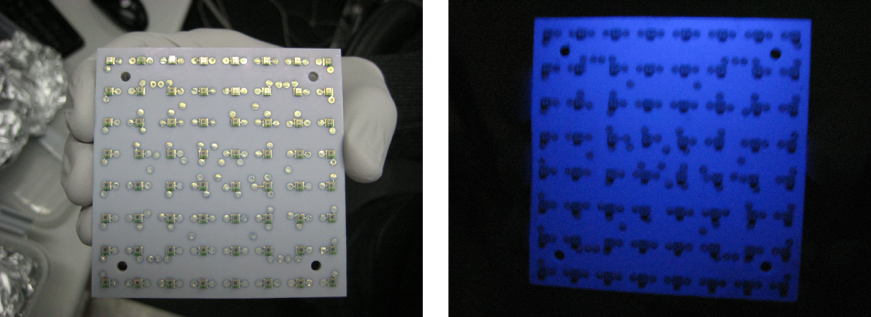
\includegraphics[scale=0.5]{img/DC.png}
	%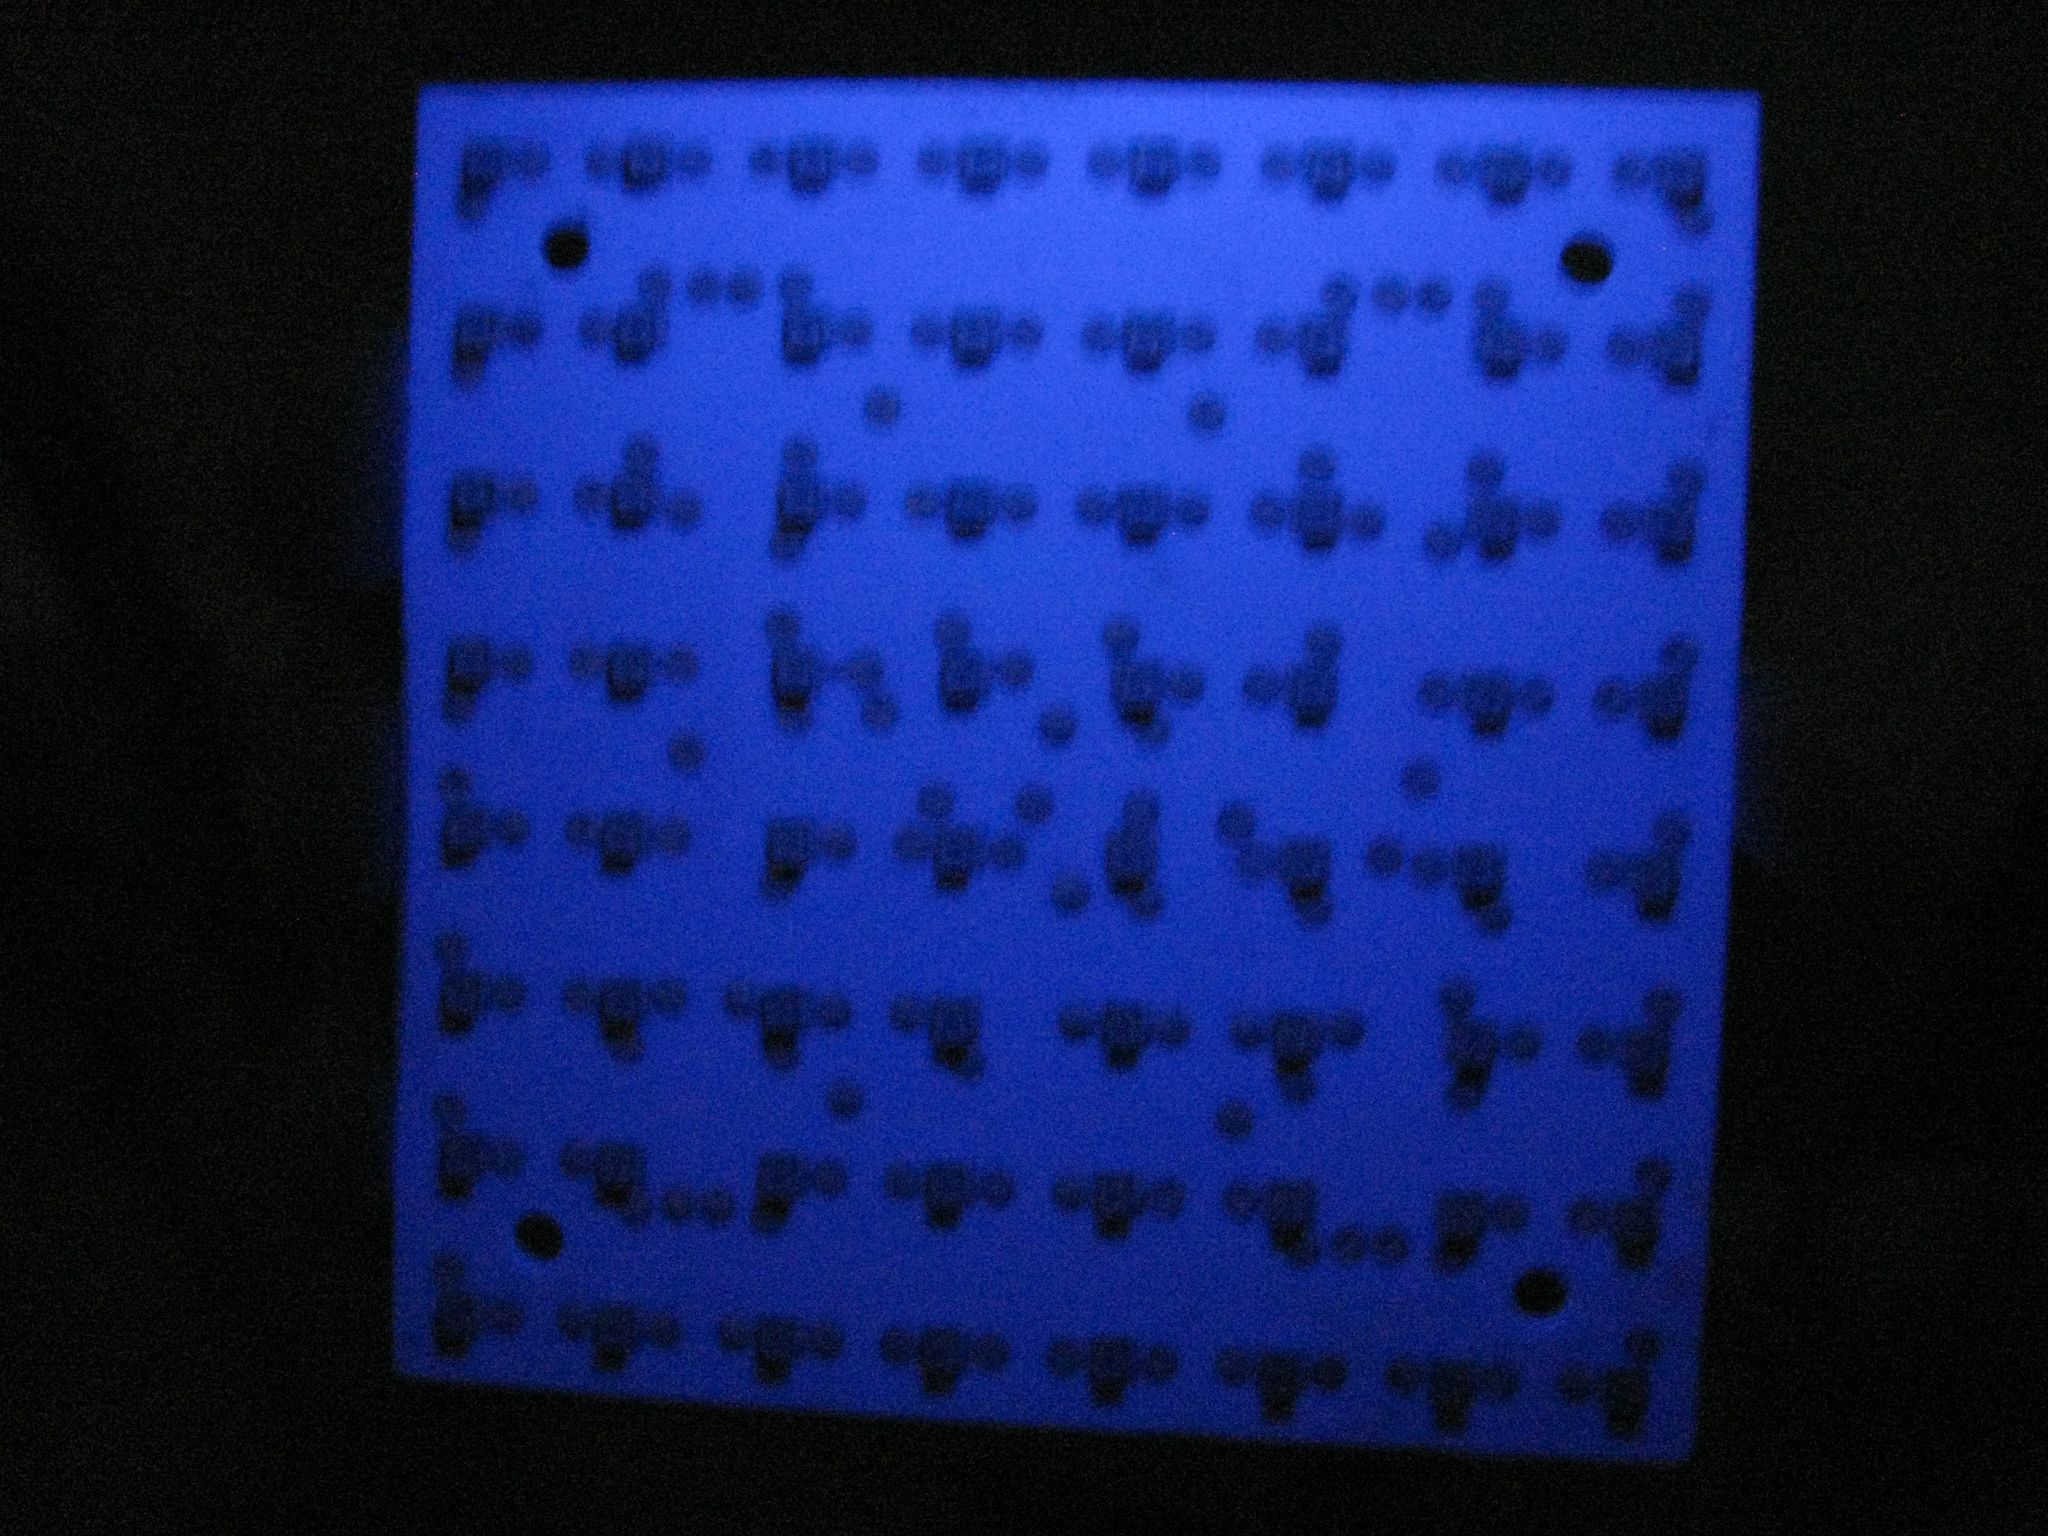
\includegraphics[scale=0.10]{img/DICE_Coated.jpg}
	\caption{\label{fig.DB} The top panel shows a DB made of Cuflon, developed for the NEXT-DEMO experiment. The DB is coated with TPB, which shifts the VUV light emitted by xenon (170 nm) to blue (420 nm). The right panel shows the response of a DB (emitting blue light) when illuminated with a UV lamp.  }
\end{figure}


Figure \ref{fig.DB} (top panel) ~shows a DB made of Cuflon, developed for the NEXT-DEMO detector. The DB is coated with TPB, which shifts the VUV light emitted by xenon (170 nm) to blue (420 nm). The bottom panel shows the response of a DB (emitting blue light) when illuminated with a UV lamp. The DBs of PETALO will have a similar design, except for the use of larger SiPMs (we are currently planning to use 6mm parts, available from several vendors).
%Figure \ref{fig.KDB} (top panel) shows a DB made of Katpon (KDB), developed for the NEW and NEXT-100 detectors. The bottom panel shows the circuitry. The DBs of PETALO will be based in the NEXT-100 KDBs.

\paragraph{The Liquid Xenon Scintillating Cell (LXSC):}

\label{sec.lxsc}

\begin{figure}[!htb]
	\centering
	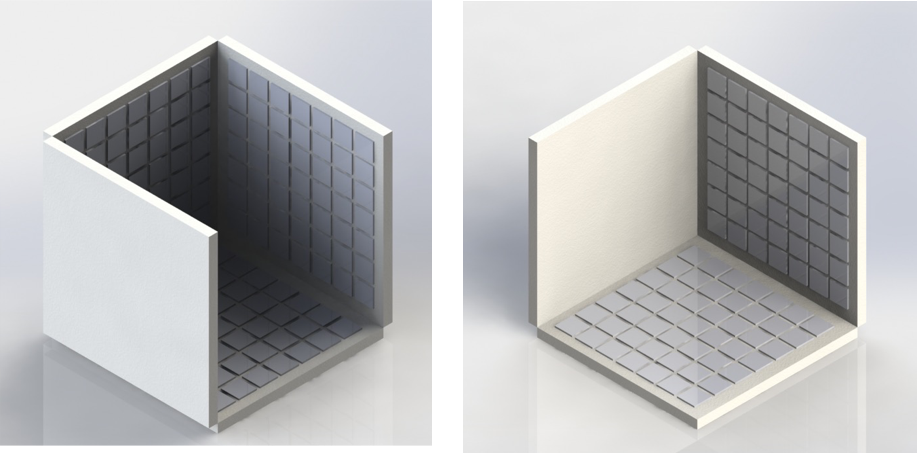
\includegraphics[scale=0.5]{img/lxsc.png}
	%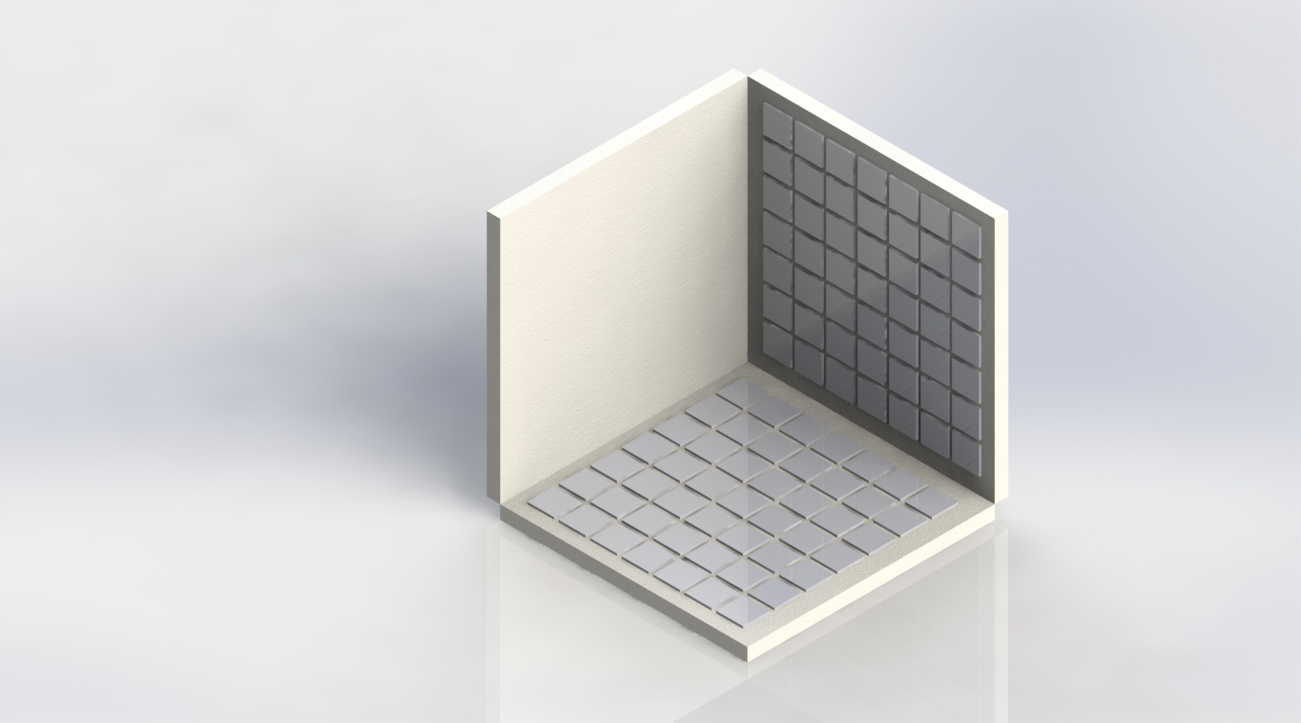
\includegraphics[scale=0.35]{img/box5open.jpg}
	\caption{\label{fig.box} The LXSC6 is a box of 
	$5\times 5 \times 5$~cm$^3$~with all its faces instrumented with SiPMs. In order to reduce costs, however, is feasible to instrument only two faces (LXSC2). The faces non instrumented are covered by reflecting teflon coated with TPB. }
\end{figure}

Figure \ref{fig.box}~shows a conceptual drawing of the keystone of the PETALO apparatus, the Liquid Xenon Scintillating Cell (LXSC). The cell is a box of $5\times 5 \times 5$~cm$^3$~ filled with liquid xenon and immersed in a cryostat. The cell transverse size (relative to the incoming beam) is optimised to minimise pileup and its longitudinal size is optimised so that most of the incoming 511 keV photons (80\%) interact in the volume. 

The best performance from the point of view of energy resolution is obtained when all the box faces are instrumented with SiPMs, as illustrated in the left panel of Figure \ref{fig.box}. We denote this configuration as LXSC6. On the other hand, the most economical configuration is obtained instrumenting only the entry and exit faces (relative to the beam direction). We call this configuration LXSC2. 
%Other possible configurations instrument three faces (entry, exit and one of the lateral faces, LXSC3) or four faces (entry, exit and two opposite laterals, LXSC4). 
The faces non instrumented are covered by reflecting teflon coated with TPB. Our Monte Carlo studies indicate that an excellent performance can be obtained even with the most sparse configurations (LXSC2). The experimental study of the detailed performance of these alternative configurations is one of the goals of this proposal.  

\paragraph{Monte Carlo simulations of the LXSC:}

%\begin{figure}[!htb]
%	\centering
%	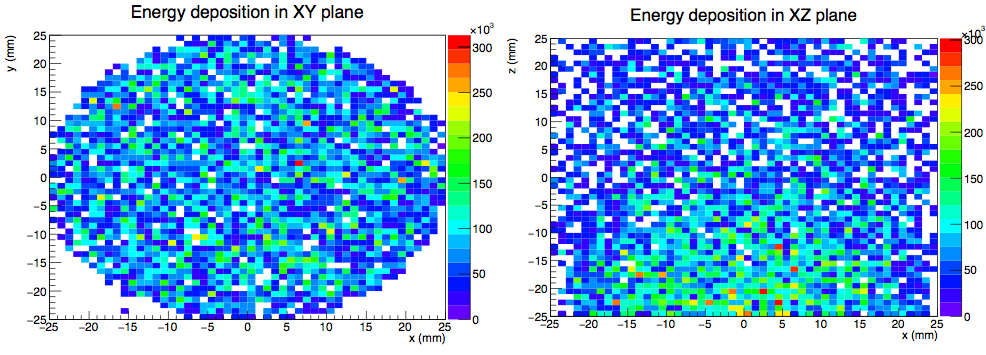
\includegraphics[scale=0.5]{img/gammas.png}
%	\caption{\label{fig.gammas}  Left panel: (x,y) distribution of the gammas interacting in the LXSC. Right panel: (x,z) distribution, showing an accumulation of interactions in the first 3 cm.  }
%\end{figure}

A full GEANT4 simulation has been carried out to study the performance of the various configurations of the LXSC. Photons of 511 keV enter the LXSC from outside (defining the ``entry face'') and interact in the cell 
%(see Figure \ref{fig.gammas}), 
through photoelectric (around 20\% of the times) or Compton interactions. About 60\% of the incoming gammas deposit their full energy in the LXSC. 

If $E$~ is the energy deposited by the ionising radiation (in this case 511 keV), the maximum scintillation yield of LXe is given as $E/W_{ph}$, where $W_{ph}$~ is the average energy required for the production of a single photon. The most probable value of $W_{ph}$~ in LXe  is\footnote{E. Aprile and T. Doke, Liquid Xenon Detectors for Particle Physics and Astrophysics, Rev. Mod. Phys. 82 (2010) 2053–2097, [arXiv:0910.4956].} is $13.8 \pm 0.9$~eV. Therefore, a maximum of 37,000 scintillation photons are produced when a 511 keV gamma interacts in the LXe. On the other hand, measurements carried out with electrons of 1 MeV result in a lower value of $W_{ph}^e = 21.6$\footnote{T. Doke, A. Hitachi, J. Kikuchi, K. Masuda, H. Okada and E. Shibamura: Jpn. J. Appl. Phys. 41 (2002) 1538.}. This lowest value is attributed to ionisation electrons that do not recombine, and would imply a yield of $\sim$ 24,000 scintillation photons for a 511 keV gammas. It turns out, in fact, that our LXSC can measure precisely the value of $W_{ph}$~ in LXe. The results presented below are obtained assuming the maximum scintillation yield, but we also discuss the implications of a lowest scintillation yield in the energy and spacial resolution. 

\paragraph{Energy resolution of the LXSC:}

The VUV photons produced by the interactions of gammas in the LXSC are shifted to 420 nm by the TPB which coats the teflon panels and the SiPMs. The conversion efficiency, measured, among other authors by the NEXT collaboration is 80\%. The resulting blue photons are registered by the SiPMs, with high efficiency (the typical PDE of modern SiPMs for 420 nm exceeds 50\%). 

While the fast decay time of scintillation (2 ns) allows for TOF applications (see below), the longer time associated with the recombination of electrons (45 ns) implies integration times of the order of 200 ns, similar to those used by LSO detectors. 
%The dark current of the SiPMs and the electronic noise of the subsequent electronics (described later in this proposal) is very low due to the cryogenic operation, and thus the resolution is dominated by photoelectron statistics. 

\begin{figure}[!htb]
	\centering
	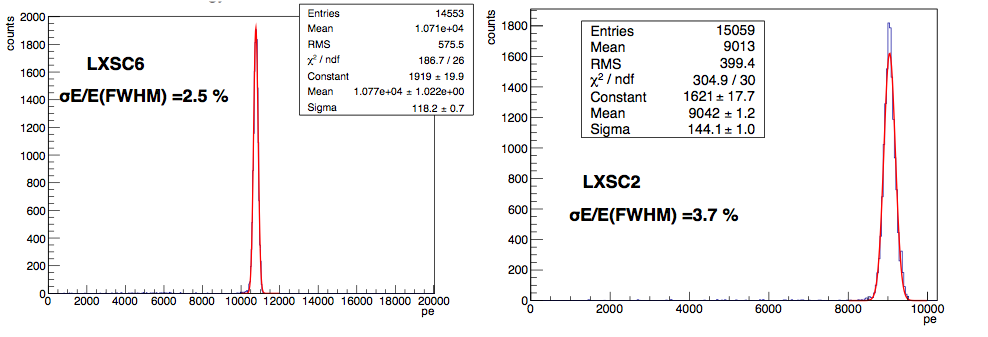
\includegraphics[scale=0.5]{img/energyResolution.png}
	\caption{\label{fig.energy}  Left panel: the intrinsic energy resolution of the LXSC6 is excellent (around 2.5\% FWHM) due to the high photoelectron statistics. Right panel: the most sparse configuration, LXSC2 records less light, but the resolution is still very good (3.7\% FWHM). }
\end{figure}

Figure \ref{fig.energy} (left panel) shows the recorded number of photoelectrons in the LXSC6 corresponding to photoelectric interactions. The fit shows a resolution of 2.5\% FWHM, {\em much better} than the resolution obtained with conventional SSDs (for example, the best resolution obtained with test systems for LSO crystals is in the vicinity of 9 \% FWHM, while commercial PETs typically show a resolution of around 20 \% FWHM). The right panel shows the recorded number of photoelectrons in the LXSC2 corresponding to photoelectric interactions ($\sim$ 9000 P.E., to be compared with $\sim$ 12000 P.E. for the LXSC6). The  fit yields a resolution of 3.7\% FWHM. If we assume the lowest $W_{ph}$~measured for electrons, the yield would be reduced by 65\% and the resolution of the LXSC2 would be around 5.5\% FWHM, which still beats by far that of modern SSDs. Indeed, the most conservative scenario for the LXSC results in a light yield similar to that of NaI SSDs, which achieve resolutions in the range of 6-7\% FWHM. Notice, however, the the slow constant decay of NaI (230 ns) makes it hardly competitive with LXe. 

%\begin{figure}[!htb]
%	\centering
%	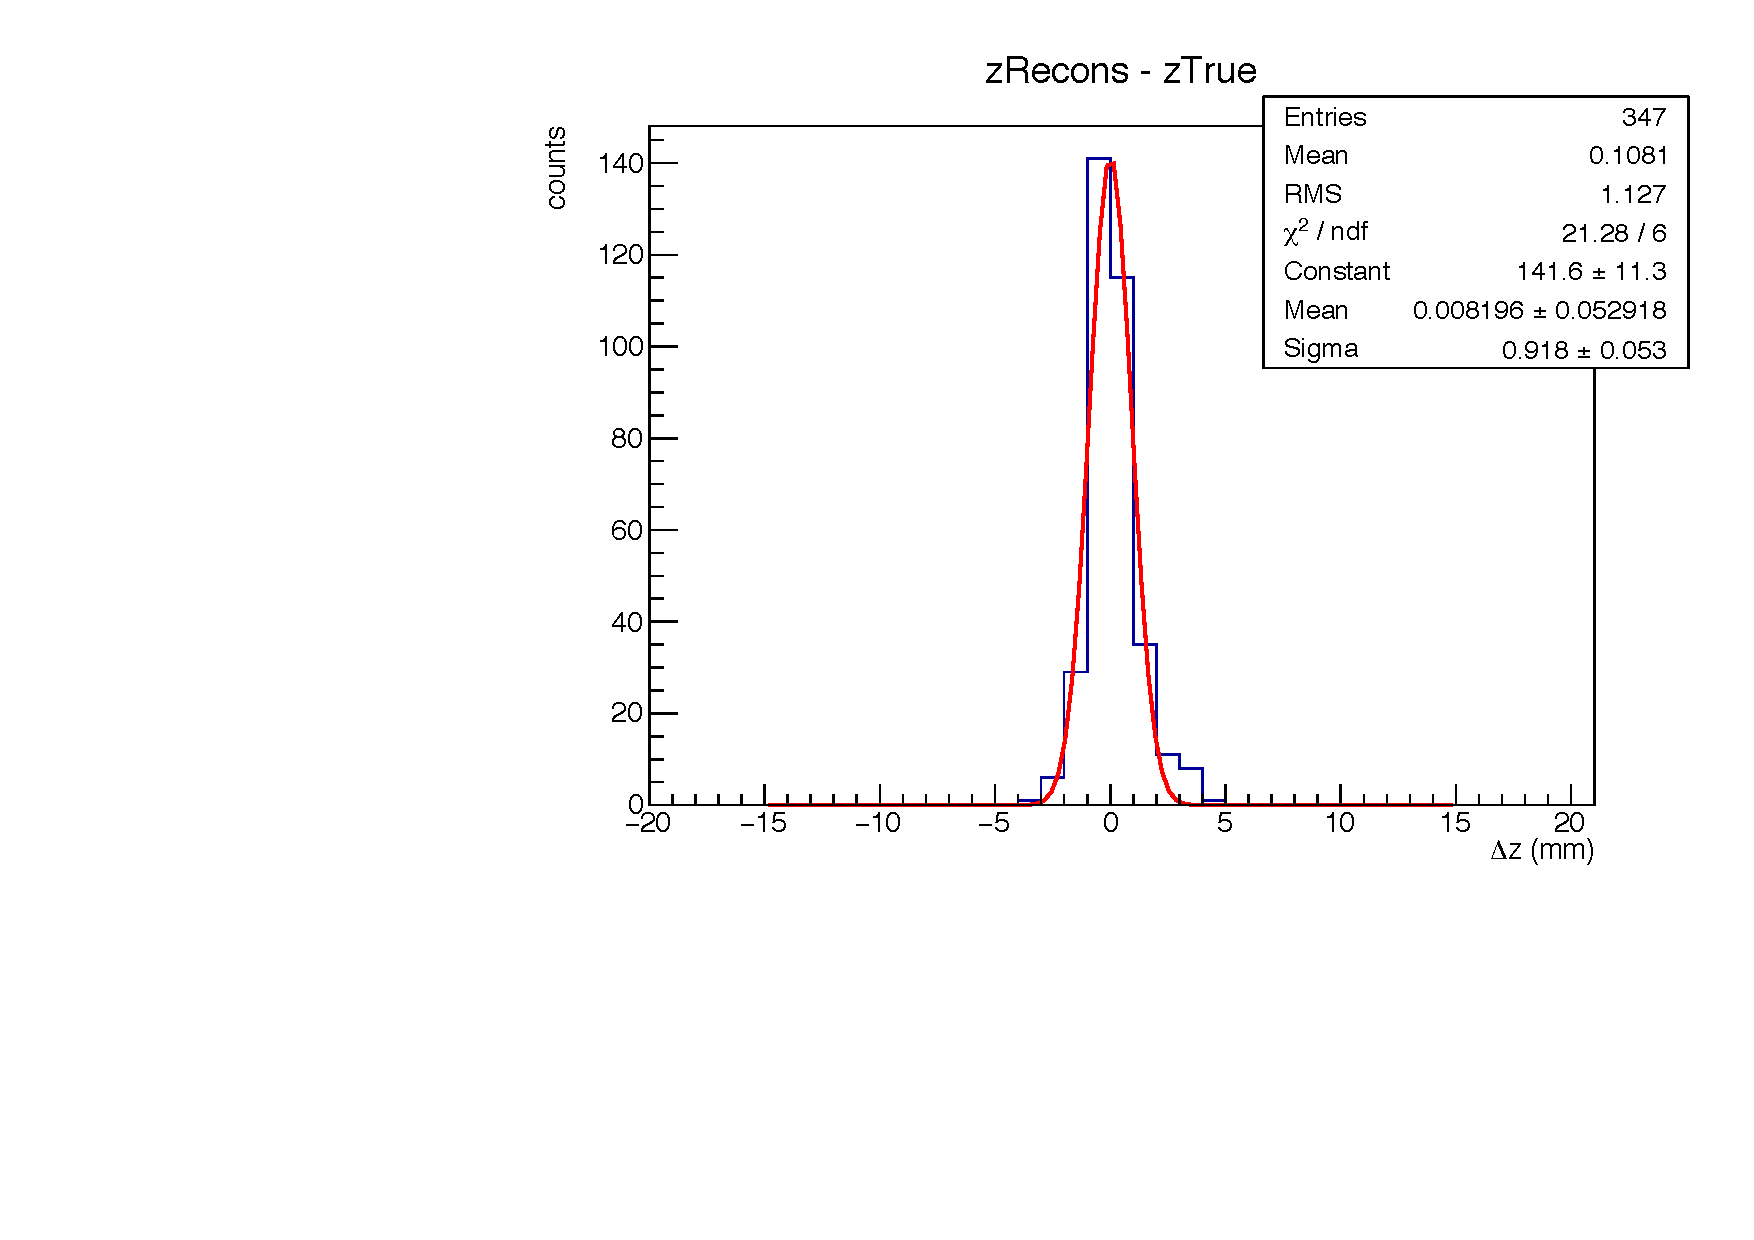
\includegraphics[scale=0.6]{img/zBest.pdf}
%	\caption{\label{fig.zbest}  Spacial resolution in the longitudinal coordinate ($z$). The transverse resolution is of the same order.  }
%\end{figure}

\paragraph{Spatial resolution of the LXSC:}
The simplest way to determine the point of interaction of an incoming photon, $(x,y,z)$~ is to use a barycentre algorithm. 
\[
\xi_r = \frac{\sum \xi_i N_i}{N}
\]
where $\xi_r$~stands for each one of the three coordinates ($x_r, y_r, z_r$), $N_i$~is the number of photoelectrons registered in each SiPM and $N=\sum N_i$. In the LXSC6  configuration one can compute redundant measurements of $\xi_r$~for each coordinate. In the  LXSC2 one can obtain ($x_r,y_r$) redundantly from the information found in the entry and exit faces and $z_r$~from the ratio of energy measured in the entry and the exit faces. 

The space resolution obtained for the LXSC6 is better than 1 mm, which is of the same order of that attained by the best conventional SSDs equipped with SiPMs. The resolution in the LXSC2 is better than 2 mm in the transverse coordinates ($x,y$) and 1.5 mm in the longitudinal coordinates.  In addition, the resolution is achieved {\em in the three coordinates}, while we recall that conventional scintillators typically do not measure well the $z$~coordinate, a fact that introduces parallax errors. 


\paragraph{PETALO as TOF-PET system:}

%\begin{figure}[!htb]
%	\centering
%	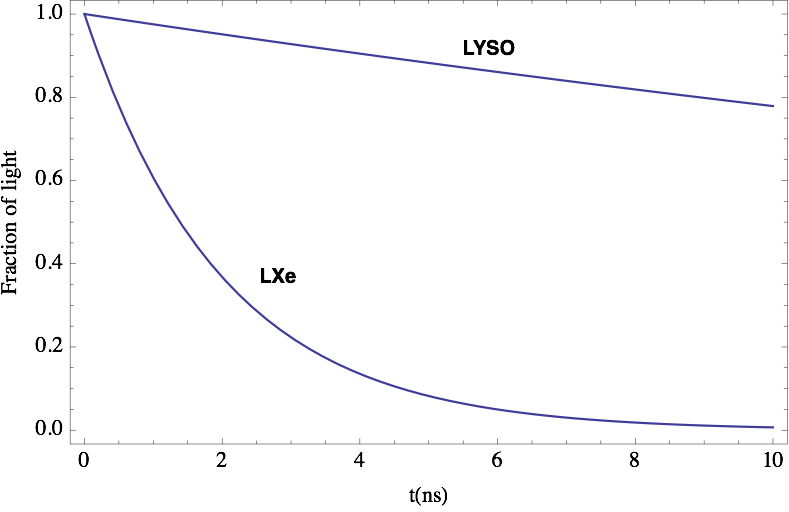
\includegraphics[scale=0.5]{img/TOF.png}
%	\caption{\label{fig.tof}  Decay time of LSO and LXe.  }
%\end{figure}

The quick decay time of xenon and the fast circuitry available in modern SiPMs offers an extraordinary potential for TOF applications. About 2.5\% of the photons are emitted in LXe in the first 50 ps after the interaction. The SiPM recording more signal in one event sees typically  2\% of the total photoelectrons (pes), and therefore it records 5 pes in the first 50 ps, enough to trigger a signal. For comparison, one nanosecond is needed in LSO to emit 2.5\% of the photons. Commercial TOF-PET systems based in LYSO (a proprietary version of LSO) have achieved a system time resolution of 600 ps. Since LXe features {\em both} higher light yield and much faster time response, a system resolution at the level of 200-250 ps appears possible, as shown by the pioneer work of the Waseda group. Thus PETALO could represent a break through in the field of PET-TOF. 

\paragraph{Resolving Compton interactions:}
Photoelectric interactions are a relatively small fraction of the total number of interactions in LXe (22\%) as well as in SSDs (for example, 33\% in LSO). The bulk of Compton interactions can result either in contained (when the scatter gamma produces a cascade that does not escape the detector) or non contained events. Non contained events do not deposit the full energy of the gamma in the detector and can be rejected. However, the large fraction of contained Compton events (60\% for the LXSC and larger for denser SSDs, such as LSO) introduce a significant distortion of the position in the case of conventional SSDs. Recall that conventional SSDs do not measure the $z$~(longitudinal) coordinate, introducing parallax errors. In addition, when a multiple-site Compton interaction occur in the detector, the transverse ($x,y$) coordinates are distorted, since the system only measures the average coordinate (many modern SSDs are very dense and thus the photon fly path is very short). 

Instead, in the LXSC, multiple-site hits are easily identified (the system measures true 3D points), and can be separated to a distance of the order of the detector pitch. This capability of separating photoelectric and Compton events can be further exploited in the case of 2-site Compton interactions. Resolving the position and the energy of both gammas with good resolution, allows the LXSC to operate as a {\em Compton Telescope}, taking advantage of Compton kinematics to further restrict the point of emission of the photons. 

\paragraph{Nuclear Magnetic Resonance compatibility:}

The LXSC  is built using non-magnetic materials, and unlike PMTs, SiPMs can operate in very high magnetic fields. Therefore PETALO can operate inside the very intense magnetic field generated by NMR devices. Furthermore, a NMS apparatus requires a large cryostat which can also accommodate the LXSC modules that make up PETALO. The technology offers, therefore, the possibility of building a fully NMR compatible device.  

\paragraph{Summary: PETALO, a break through in PET technology:}
To summarise, the PETALO concept offers the following advantages:
\begin{enumerate}
\item Light yield higher than any conventional SSD.
\item Excellent energy resolution (2.5 -- 5 \% FWHM, depending on configuration of LXSC and of light yield). 
\item Excellent spatial resolution (1-2 mm in the three coordinates, minimising parallax error).
\item Capable of detecting multi-site Compton events. Thus suitable as Compton telescope.
\item Very fast time response, resulting in enhanced sensitivity (reduced number of random coincidences) and making it possible a break-through TOF application. 
\item Fully NMR compatible. 
\item Competitive cost. The LXSC2 version of PETALO would cost today roughly half of the cost of the equivalent LSO unit. With the cost of SiPMs falling, the  cost of PET scanners will soon be fully dominated by the material of choice. Xenon is much cheaper than LSO and thus a large-scale apparatus (full body PET) is conceivable. 
\end{enumerate}


\subsubsection*{Previous work }

%PETALO is a clear case of direct transference of the technology developed in the context of an experiment related with fundamental research in particle physics (the search for neutrinoless double beta processes), to a medical imaging application with the potential of leading the field in several aspects (energy resolution, full 3D imagining within the detectors, capability of resolving Compton interaction, excellent time resolution providing unsurpassed TOF capabilities and compatibility with NMR).  

The previous work of the teams participating in this proposal, relevant to this project, can be summarised as follows:

\subsubsection*{IFIC group. Technology transfer from the NEXT collaboration}

The \emph{Neutrino Experiment with a Xenon TPC} (NEXT)\footnote{http://next.ific.uv.es/next/} will search for neutrinoless double beta decay processes (\bbonu) in \XE\ using a  high-pressure xenon gas time projection chamber. The design of the NEW (the first stage of the experiment, deploying 10 kg of enriched xenon) and NEXT-100 (second stage, deploying 100 kg of \XE) detectors is optimised for energy resolution by using proportional electroluminescent (EL) amplification of the ionisation signal. The detection of EL light provides an energy measurement using photomultipliers (PMTs) located behind the cathode (the \emph{energy plane}) as well as tracking through its detection a few mm away from production at the anode, via a dense array of silicon photomultipliers (the \emph{tracking plane}).

\begin{figure}[!htb]
	\centering
	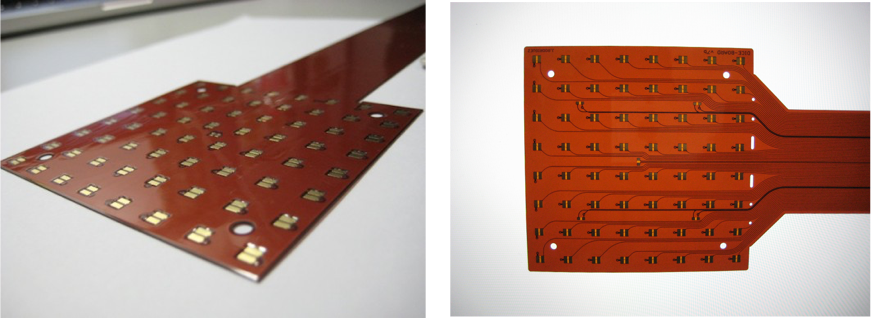
\includegraphics[scale=0.5]{img/KDB2.png}\\
	\caption{\label{fig.KDB} Top and bottom pictures of the Kapton Dice Boards (KDB) developed for the tracking plane of the NEW and NEXT-100 detectors by the NEXT collaboration.}
\end{figure}

In NEW and NEXT-100 the tracking function is provided by a plane of SiPMs operating as light-pixels and located behind the transparent EL grids. They are mounted on flexible radiopure Kapton Dice Boards (KDBs). Each KDB hosts 64 SiPMs (Figure  \ref{fig.KDB}). The NEW  tracking plane is currently being commissioned with 28 KDBs. The NEXT-100 tracking plane will deploy 112 KDBs.  

The dice boards for the LXSC will be built using the technology developed by NEXT. The design is essentially the same, since the SiPMs foreseen for PETALO are of the same type deployed by NEW and NEXT-100 (SENSL C or J series). The main difference is the size of the SIPM (6 mm rather than 1 mm) which however affects very little the design. 

The NEXT KDBs have been developed by the IFIC group during a period of five years. Currently the technology and expertise of the group is very mature and can be reused at a very moderate cost both in terms of money and personnel. 

%PETALO is a liquid-xenon, scintillation based detector with a simpler design and operating conditions  that the NEXT-DEMO, NEW and NEXT-100 detectors. It does not operate at high pressure and does not involve electric fields. Cryogeny at LXe temperatures is rather straight forward and the purification of the gas system much simpler than in the case of NEXT. It will fully benefit from the experience acquired over the last seven years by the IFIC NEXT team. 

\subsubsection*{I3M-UPV group: expertise in the development of ASICS for PET}

The I3M-UPV research team has developed two ASICs for PET applications that
exploit the benefits of analog processing and reduce the number of channels
to acquire thus cutting down the complexity of the following DAQ system. 
The first of them, PESIC\footnote{Herrero-Bosch, V. et al., 
``PESIC: An integrated Front-end for PET
Applications'', Nuclear Science, IEEE Trans. on, vol.55, 2008.} was designed to work mainly with multi-anode
Position Sensitive Photomultiplier Tubes (PSPMT). Its architecture was
designed to improve time behaviour and increase spatial resolution. Its
preamplifying stage introduced two main benefits: digitally programmable gain
adjustment for every photomultiplier output, and isolation from front-end
electronics by means of current buffers. This last feature allows using
different types of photomultipliers such as SiPM and optimises front-end
dead-time, reducing impact position dependent output delay. PESIC used a
resistive charge division network to obtain bi-dimensional information of the
detected event inside a scintillation crystal.  Individual gain control of
the inputs introduced a calibration mechanism close to the detector. This
fine tuning capability improved its overall performance by minimising gain
deviations along the PSPMT sensitive area\footnote{Herrero-Bosch, V et al. ``Position sensitive scintillator based detector
improvements by means of an integrated front-end'', Nuclear Instrument and Methods
A, no.604, 2009.}. However PESIC architecture
was limited to 64 inputs and could not be easily scaled to a higher number
of inputs.

The second ASIC, AMIC\footnote{Herrero-Bosch, V. et al., ``AMIC: An Expandable Front-End for Gamma-Ray
Detectors With Light Distribution Analysis Capabilities'', Nuclear Science,
IEEE Trans. on , vol.58, no.4, 2011.} shared with PESIC a preamplifier stage but carried
out a more complex operation with the inputs. Its unique architecture
allowed carrying out up to 8 parallel calculations with these inputs in the
analog domain. These operations consist of a scaling by an 8 bit precision
digitally configurable coefficient for every input and a sum of the results.
Each one of the fully analog blocks which implemented this basic operation
was named CB (Computational Block). Inside each CB a different set of
coefficients can be programmed so that it can calculate the geometrical
moment of the light distribution obtained from the photodetector. Zero order
moment can be identified with total energy; first order moment is related to
the baricenter of the light distribution and so on. Since the basic
operation is an additive one, the underlying principle of the architecture
can be extended to an arbitrary number of inputs using several AMIC devices
with the right set of coefficients programmed inside. The upper limit of
devices being employed is only limited by the required Signal to Noise Ratio
(SNR). The value of the coefficients may include any calibration needed to
optimise detectors response\footnote{Herrero-Bosch,V.; et al., ``Programmable integrated front-end for
SiPM/PMT PET detectors with continuous scintillating crystal'',
Instrumentation, Journal of , vol.7, Dec. 2012.}. AMIC design was fully developed up to the
industrial level and produced in medium scale for a Spanish medical imaging
company.

\subsubsection*{Expertise of the GIBI230-LaFe group}

The Principal Investigator and the members of the research group form a multidisciplinary team including physicists, nuclear physicians and telecommunications engineers inside the Biomedical Imaging Research Group GIBI230\footnote{http://www.iislafe.es/biomedica-imagen.aspx} . Their experience include:
\begin{enumerate}
\item Development and validation of imaging biomarkers.
\item New techniques and diagnosis based in molecular imaging.
\item Combined analysis of molecular and anatomical information.
\item Definition and implementation of parametric imaging including biological, functional and anatomical information.
\item Safety aspects regarding the use of ionising radiation. 
\end{enumerate}



\subsubsection*{Objetivos generales y adecuación al Programa Estatal de I+D+i orientada a los Retos de la Sociedad / General objectives and match to the National Programme for research aimed at the Challenges of Society}

\paragraph{Overall objectives.}
The overall objectives of this research proposal are:

\begin{enumerate}
\item Construction, commissioning and characterisation of the PETALO-2  (P2) prototype. %Demonstration of the energy resolution and spacial resolution of the LXSC. Study of the performance of several configurations (LXSC2, LXSC3, LXSC6). Demonstration of coincidence resolution time (CRT) between the two LXSC of P2. Characterisation of photoelectric and multi-site, fully contained Compton events. 
\item Development of FE electronics and DAQ optimised for P2. 
\item Construction, commissioning and characterisation of the PETALO-10 (P10) small animal PET in a non-clinical environment.
\item Development of FE electronics and DAQ optimised for P10.
\item Characterisation and study of performance of P10  in a clinical environment.  
\item Operation and optimisation of  P10 in a NMR environment.
\item Image processing and reconstruction combining PET and NMR data. 
\item Optimisation of  P10 as TOF-PET apparatus.
\end{enumerate}

The objectives presented in this project are very well aligned to the Spanish program for science. They involve a direct technology transfer from a basic science experiment in particle physics to a medical imaging application of high social impact. It involves a multidisciplinary collaboration between physicist, engineers and medical doctors. And it has a large potential for generating commercial spinoffs, including the possibility of a break through in the PET technology.  




%\input{src2/RETO6.tex}

\subsubsection*{Objetivos específicos / Specific objectives}
%

\input{src/ObjDet.tex}
\input{src/ObjAsic.tex}
\input{src/ObjImg.tex}

\subsubsection*{Metodolog\'ia / Methodology}

%4. El detalle de la metodologia propuesta en cada uno de los subproyectos participantes
%The specific objectives of all the subprojects are integrated in the PETALO Project Management Plan (PMP). The PMP coordinates the construction of P2 and P10 detectors. It is under the direct supervision of the Spokesperson (SP), the Medical Spokesperson (MSP), the Project Manager (PM) and the Medical Project Manger (MPM), and links with the PIs of this project\footnote{The PETALO SP is Prof. J.J. Gómez Cadenas; the MSP is Dr. Luis Martí-Bonmatí; the PM is Prof. J. Toledo; the MPM is Dr. Ángel Alberich. The collaboration steering committee includes the SP, MSP, PM, MPM and the PIs of the three projects presented here}. 

The PMP defines rigorously the activities (also called working packages WP) of the project and follows the progress of each one, monitors deliverables and deadlines and keeps track of invested resources including personnel. It also identifies potential show-stoppers and synergies (and possible conflicts) between the different projects and optimises the sharing of resources. 

%Figure \ref{fig.Gantt} shows an example of the Gantt chart for the whole NEW project, up to installaton at the LSC. 

%The objectives defined for the different sub projects match the various WP in the PMP, as can be seen in Figure \ref{Fig:PMP}. 

The methodology of each WP includes: a) the definition of the associated tasks; b) the identification of the resources needed; c) the temporal organisation of the tasks; d) the definition of milestones and the deliverables associated to them; e) the relations with other WP. Each WP has a leader, which reports directly to the PM/MPM. The progress of each WP is reviewed on a weekly basis. Milestones and potential showstoppers are discussed, and the tracking charts updated if needed. 
\subsubsection*{Methodology of the DET subproject}

\paragraph{Construction and commissioning of P0 and P4:}

\begin{figure}[!htb]
	\centering
	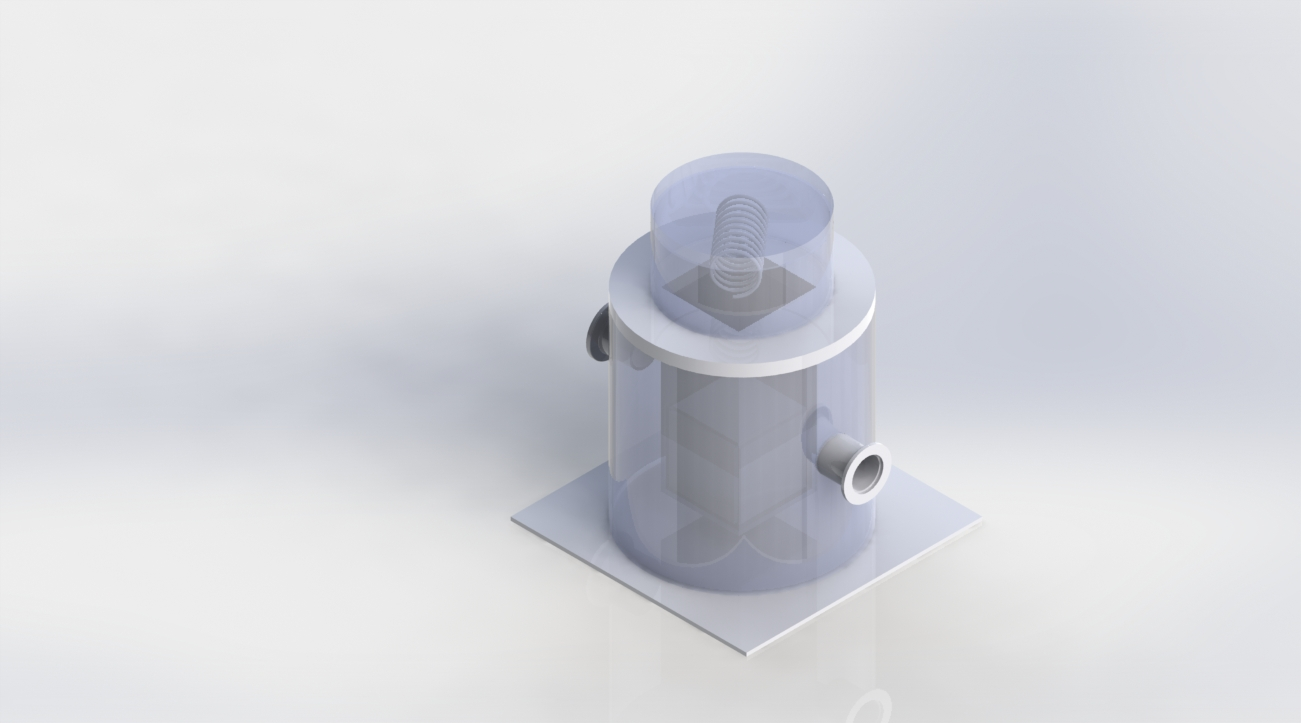
\includegraphics[scale=0.35]{img/PETALO-0.jpg}
	\caption{\label{fig.P0} Conceptual sketch of P0.  }
\end{figure}

\begin{figure}[!htb]
	\centering
	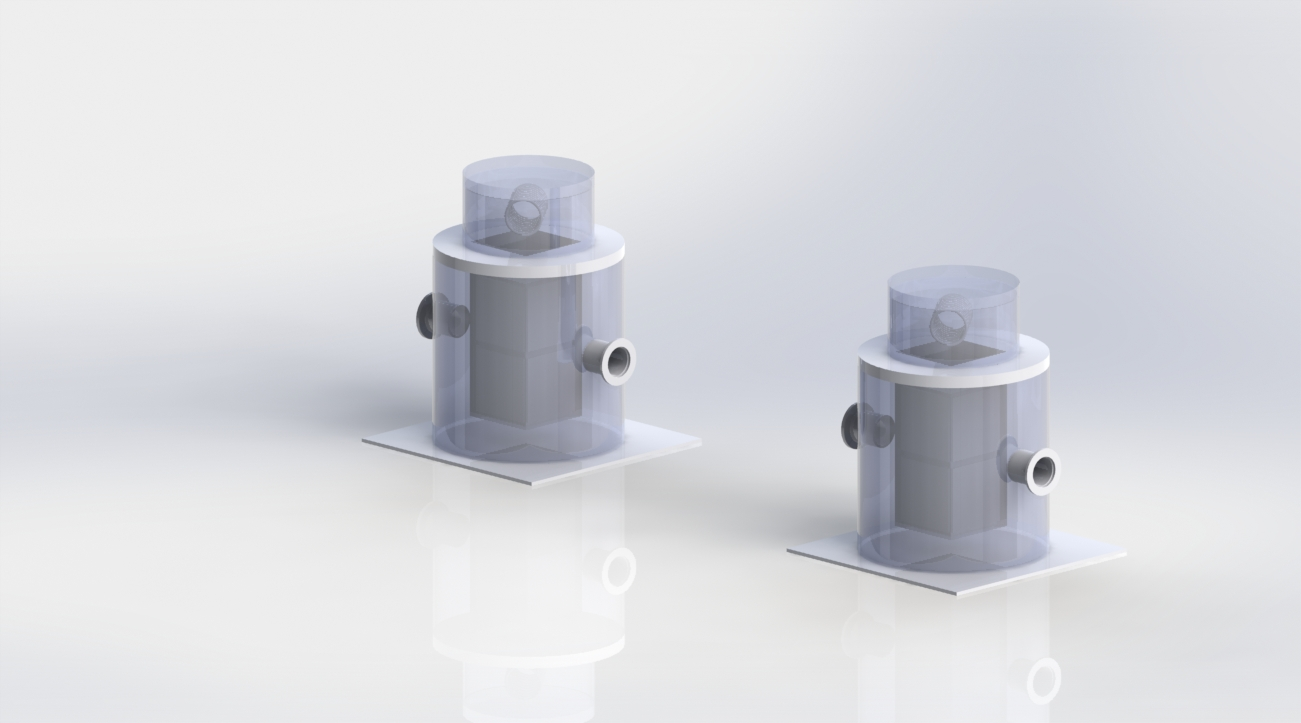
\includegraphics[scale=0.35]{img/PETALO-4.JPG}
	\caption{\label{fig.P2} Conceptual sketch of P4. }
\end{figure}

PETALO-0 (P0) will be a demonstrator used to study the intrinsic performance of the LXSC. Figure \ref{fig.P0} shows a conceptual sketch. A fully instrumented LXSC6, immersed in its own cryostat will be studied with a radioactive source emitting 511 keV photons, such as Na-22 (eventually other sources will be used to study the linearity of the system). The redundancy of LXSC6 will allow to measure the energy and spatial resolution from the data themselves. In addition, P0 will be used to understand the energy and time triggers of the device. 

PETALO-4 is a demonstrator of the PETALO concept using 4 LXSC arranged in groups of two, facing each other. The system can be designed with two independent cryostats (each cryostats holds two cells), as shown in Figure \ref{fig.P2} to permit maximum flexibility in the placement and arrangement of the device. P4 will be used to reconstruct images from phantoms and eventually small animals, in order to demonstrate the imaging reconstruction capabilities of PETALO as well as its potential as TOF device. 

%\begin{figure}[!htb]
%	\centering
%	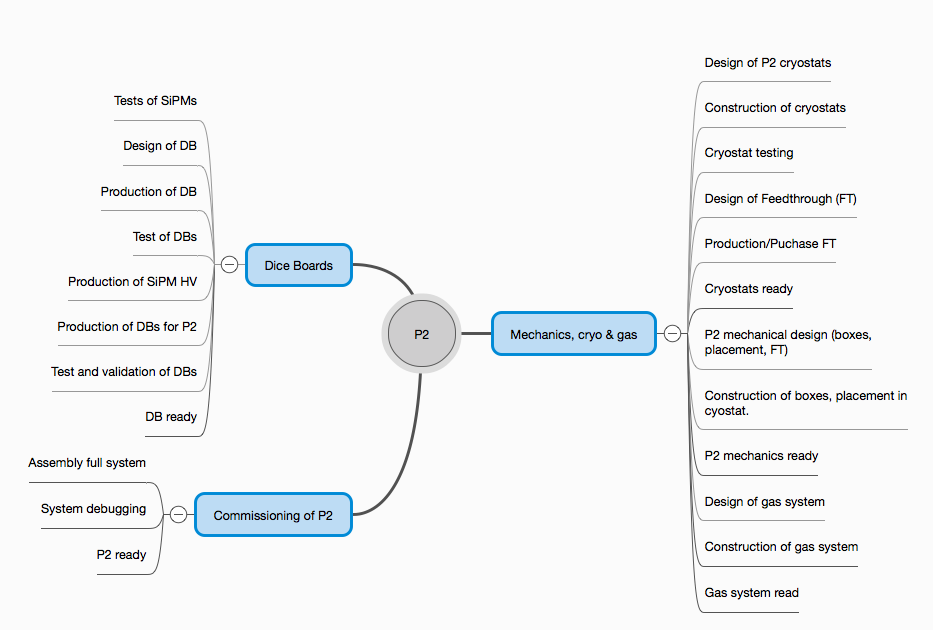
\includegraphics[scale=0.5]{img/P2MIND.png}
%	\caption{\label{fig.P2MIND} Conceptual breakdown of activities for the construction of P0 and P4.  }
%\end{figure}

\begin{figure}[!htb]
	\centering
	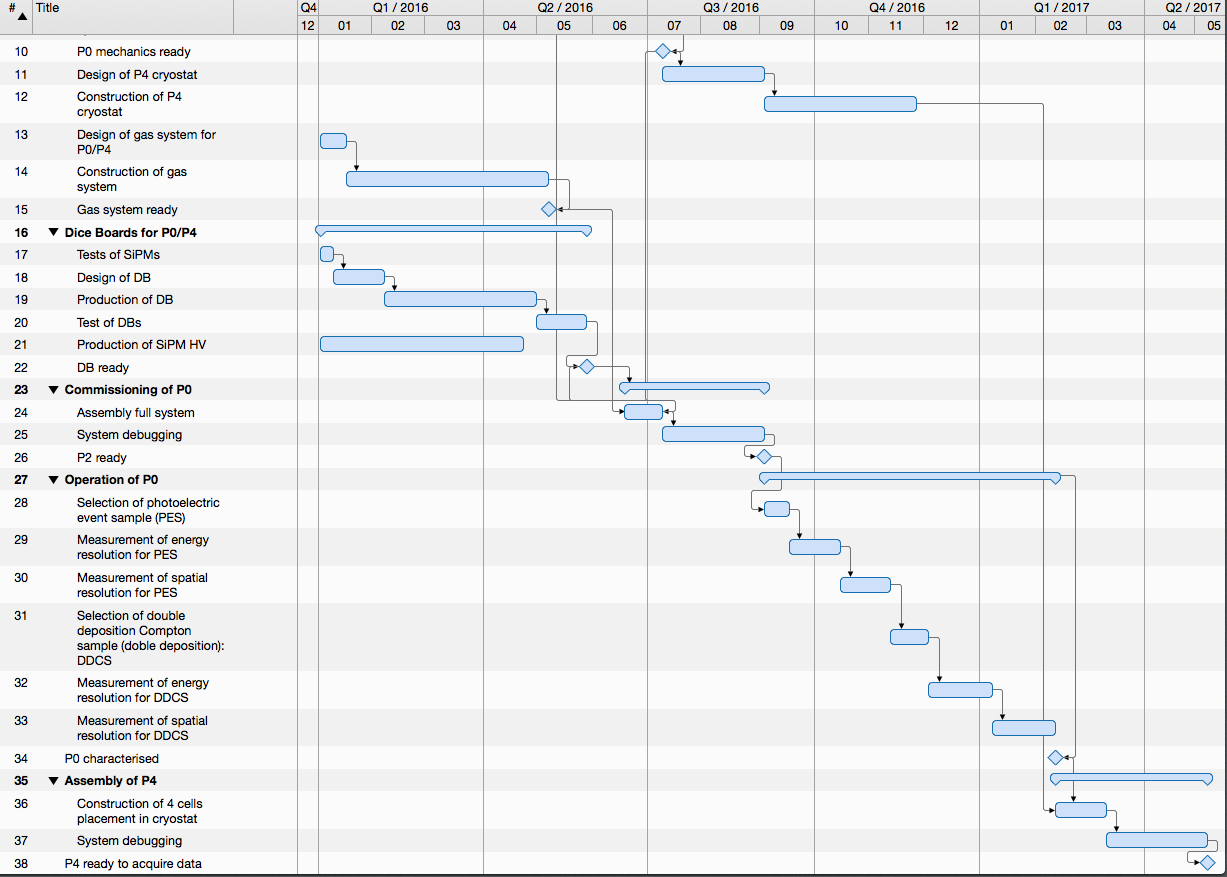
\includegraphics[scale=0.4]{img/PDETWF.png}
	\caption{\label{fig.P2WF} Work flow of activities for P2/P4.  }
\end{figure}

The construction of P0 and P4 involve a number of activities  organised in three groups: (i) Mechanics, cryogenics and gas system (MCG);  (ii) Dice Boards for P0 and P4 (DB);  and assembly, commissioning and operation (ACP) for P0 and P4. 

The MCG group includes the design, construction and tests of the cryostats; the design and construction of the feedthroughs (FT) needed to extract the signals from the DB to the digitising electronics located outside the cryostats (the FT will be of the same time used for the NEXT tracking plane and manufactured by the same company that was employed by NEXT);  and the design and construction of ancillary mechanics. The DB group includes the design, production and test of the DB (which will be straight-forward modifications of the DB used in the NEXT tracking plane, and manufactured by the same company employed by NEXT), the production of the SiPM high-voltage modules (these have been developed by NEXT and PETALO will only need to pay for an extra production of modules), and the testing and assembly of the full system. The ACP group includes the activities related with the commissioning and operation of the devices. A detailed work flow (WF) is shown in Figure \ref{fig.P2WF}. The WF, including dependencies of tasks yields a schedule for the construction of P2 that encompassed the first two quarters of 2016 (we denote this as Q1/Q2-16). 

\paragraph{Operation of P0:}

%\begin{figure}[!htb]
%	\centering
%	\includegraphics[scale=0.5]{img/EnergyCor2P2.png}
%	\caption{\label{fig.ECP2} Dependence of the energy measured in P2 wit the transverse (x) and longitudinal (z) coordinate. A small position dependence is observed.   }
%\end{figure}

P0 will demonstrate the excellent resolution of the system in energy, position and time. A \NA\ source, located between the two modules will emit back-to-back gammas, which will be the primary calibration source of the detector. 

\paragraph{Construction and commissioning of P4:}
%
%\begin{figure}[!htb]
%	\centering
%	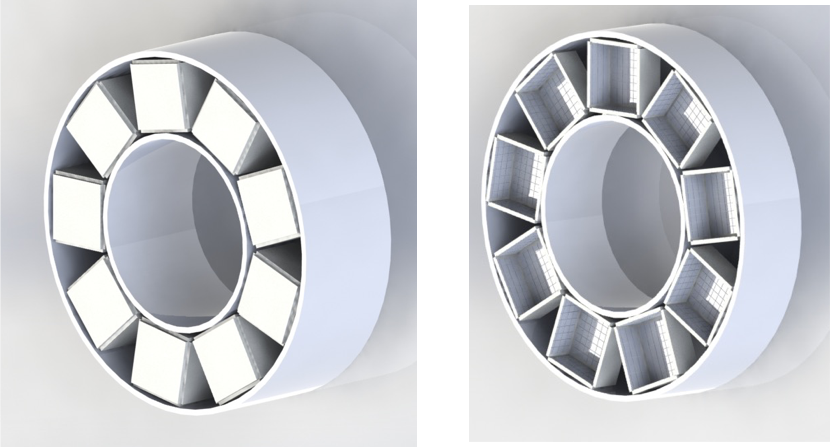
\includegraphics[scale=0.5]{img/SAP.png}
%	\caption{\label{fig.P10} Conceptual sketch of P10.  }
%\end{figure}

PETALO-4 (P4) is a proof-of-concept PET based in 4 independent LXSC2. It will allow the reconstruction of images both from phantoms and from small animals. It will be certified for its use in a hospital (La Fe, Valencia), and will be tested inside the intense magnetic field produced by the NMR research apparatus available at La Fe, to validate the potential operation of PETALO in conjunction with nuclear magnetic resonance.  

%\begin{figure}[!htb]
%	\centering
%	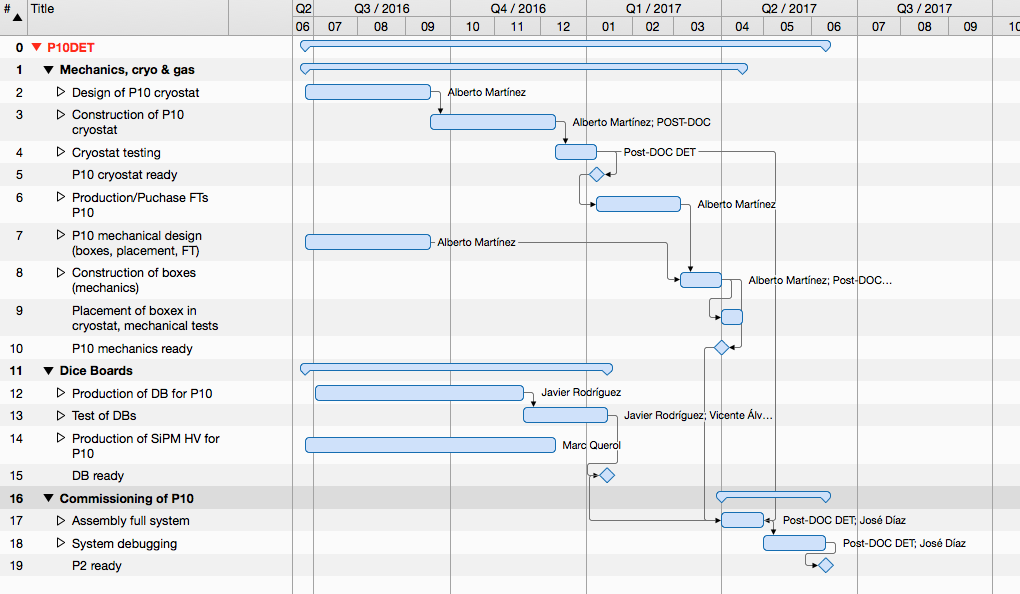
\includegraphics[scale=0.5]{img/P10WF.png}
%	\caption{\label{fig.P10WF} Work flow of activities for the construction of P10.  }
%\end{figure}

P4 will be built reusing 4 of the 6 DB of P0, and therefore only 2 additional DB (and their corresponding electronics) will be needed in addition to those deployed by P0. The construction of the device requires a second (small cryostat), and will use the same gas system than P0 and identical electronics. This permits a very fast time schedule. P0 will be built, commissioned and studied during Q1/Q3-16 and P4 will be ready in Q4-2016. 

%The cells of PETALO will be LXSC2. Production will start after the validation of the LXSC2 design with P2. The PETALO system is scalable, since all the components (DBs, electronic modules) are identical. The gas system is common with P2. The main challenge of P10 is the cryostat. The design of the cryostat will start already in 2016, and will built on the experience of the P2 cryostats. A period of six months is foreseen for the design, followed by six more months for construction. Figure \ref{fig.P10WF} shows the work flow of activities for the construction of P10, which extends from Q2-16 to Q2-17. The activities are similar to those of P2, although the development time has been adjusted to take into account the larger number of cells (DBs) and the complexity of the cryostat design/construction/commissioning. 
% 

\paragraph{SIMPLE and RAP:}
The PETALO simulation (SIMPLE) and software framework analysis (RAP) will be based in existing software developed by the NEXT collaboration. Dr. Ferrario, who has been one of the leading software and analysis developers for NEXT will be fully dedicated to PETALO starting in 2016 and will use her extensive experience to produce working versions of both SIMPLE and RAP by Q2-16. Further development will occur in parallel with the analysis of P4 data, during Q3/Q4-16. This project proposes a FPI student, who will contribute to the software and analysis development (as well as to the operation of P4) working closely with Dr. Ferrario and Prof. J. Díaz.

\paragraph{PETALO as TOF device:}
P4 will allow the measurement of the Coincidence Resolution Time (CRT) by comparing the time stamp provided by the opposite LXSC cells. A CRT in the range of 200-250 ps is expected.The IFIC group will lead the studies related with CRT determination and will participate in the studies of imaging reconstruction using TOF techniques. 

%\paragraph{DET: Summary}
%The DET subproject is in charge of the construction of the P2 and P10 apparatus, as well as of the development of some essential software tools. The construction of P2 will occur during Q1/Q2-16, while the construction of P10 will extend from Q2-16 to Q2-17. Furthermore, during the second half of 2016, P2 will be operated and the main performance parameters (resolution in energy, space and time) of PETALO demonstrated. 

%DET reuses heavily the experience and infrastructure available at IFIC from the NEXT project. The PI, prof. J. Díaz, is a NEXT collaborator, which has led several key activities in the experiment (tests of energy resolution with DEMO-0, tests leading to the choice of NEXT PMTs, among others)  and has extensive experience in nuclear instrumentation. The design and construction of the apparatus will benefit from the availability of engineering man power. The software and analysis from the experience of Dr. Ferrario who qualifies, given her unique experience to obtain a ``young researcher'' award or a Severo Ochoa grant. The project requires one additional post-doc which is requested in this grant and offers excellent formative prospects for a FPI student. 

%%\item Operation of P2 inside the magnetic field of the NMR research apparatus at La Fe. Optimisation of operation and imaging in magnetic field. This is a common objective with subproject IMG (Q3/Q4-17). 
%\end{itemize}
%\item {\bf Construction, commissioning and characterisation of the P10 small animal PET in a non-clinical environment}. 
%\begin{itemize}
%\item Construction of 10 LXSC modules, after validating the optimal configuration for P10 (Q3/Q4-17). 
%\item Construction of the P10 cryostat  and gas system (Q3/Q4-2017).
%\item Commissioning of P10 at IFIC (Q1/Q2-2018). This objective links with the subproject ASIC, since commissioning of P2 requires the availability of the FEE, DAQ and SC for P2.
%%Operation of PETALO-10 in a clinical environment with small animals. This objective is common with subproject IMG, and will be carried out by a team including scientists from both groups (Q3/Q4-18).
%\end{itemize}
%\end{enumerate}
%
%\paragraph{DET-SOFT.}
%\begin{enumerate}
%\item {\bf Development of SIMPLE}. 
%\begin{itemize}
%\item Simulation of the response of P2 (Q1-2016).
%\item  Production of simulated data for P2 studies (Q2/Q3-2016).
%\item Simulation of P10 (Q2/Q4-2016). 
%\item  Production of simulated data for P10 reconstruction studies (Q1/Q4-2017).
%\end{itemize}
%\item {\bf Development of RAP}. 
%\begin{itemize}
%\item Development of framework, event data model and software tools (Q1-2016).
%\item  Analysis of simulated data for P2 studies (Q2/Q4-2016).
%\item Analysis of simulated data for P10 studies (Q1/Q4-2017). 
%\item  Integration of imaging algorithms (Q1/Q4-2018).
%\end{itemize}
%\end{enumerate}
%
%
 
\subsubsection*{Methodology of the ASIC subproject.}

The front-end electronics (FEE) Data acquisition (DAQ) and slow controls (SC) 
for P0 and P4 will also use the solutions which have been jointly developed between NEXT, CERN and other institutions (who joined later the project) for the CERN RD-51 collaboration. We describe them briefly here. 

\paragraph{A DAQ solution for P0/P4:}
%
We propose to use the NEXT/RD-51 DAQ system, named SRS \footnote{S.Martoiu et al., JINST (8) 2013, DOI: 10.1088/1748-0221/8/03/C03015,J .Toledo et al, JINST (6) 2011, DOI: 10.1088/1748-0221/6/11/C11028.}, which has been licensed to an European company, EicSys, and ported to the industry standard ATCA.
%
The main SRS-ATCA components are: (1) An ATCA chassis, which includes power, cooling fans and a shelf manager unit for remote monitoring and control via Ethernet; (2) ATCA blades, which are carriers with mezzanine connectors, memory, processing units (FPGAs) and I/O connectivity; and (3) mezzanine cards to adapt to a wide range of front ends. Operation with the NEXT-DEMO and NEXT-NEW detectors has shown the stable and reliable operation of SRS-ATCA. 

The ADC mezzanines can achieve 60 MHz sampling rate. P0 will have one LXSC6 ($64 \times 6 = 384$~channels) and P4 will have 4 LXSC2 ($64 \times 8 = 512$~channels reusing also those previously deployed in P0).Each mezzanine handles 24 channels. Thus, 22 mezzanines will provide 528 channels.  

Each ATCA blade carries two mezzanines. So, 12 ATCA blades are required, fitting in a 12-slot  ATCA chassis. Ot these, 11 blades are used for digitisers (512 channels) and 1 blade for TDCs. The ATCA blades send data to a DAQ PC farm. Experience with the NEXT experiment, indicate that for good performance, 14 DAQ PCs would be needed (10 for Local Data Concentrators, 3 for Global Data Concentrators and one as a Storage PC). 

%
\paragraph{A solution to achieve high time resolution in P0/P4:}
%
One of the most promising applications of PETALO is to function as TOF-PET. This requires excellent time resolution. Fortunately, a ready solution also exist. In the near future, EicSys will be upgrading their ATCA blades to include WhiteRabbit\footnote{[3] http://www.ohwr.org/projects/white-rabbit} nodes in its I/O section. WhiteRabbit is a CERN development used to synchronise thousands of elements in a distributed DAQ and control system across kilometre distances with sub-nanosecond resolution. In small setups like a PET, synchronisation within 200 picoseconds can be achieved with a careful calibration process. WhiteRabbit is an extension to GbE over fibre optics and uses SFP transceiver modules.
%
%%A similar approach was developed by a former member of out research group at UPV, showing better performance in some aspects. White Rabbit is open hardware and so the firmware is freely available. Thus, we must invest effort (three months sound reasonable) in reducing as much as possible skew and jitter in the White Rabbit network, as this will be the main limitation to the time resolution in the PET. This implies potential enhancements in the synchronization protocols, in electronic componentes and in network architecture.
%
%%A Spanish company based in Granada, named Seven Solutions [ref4], develops and provides solutions based on WhiteRabbit. Apart from the WhiteRabbit nodes in the ATCA blades, which will be equipped by EicSys, we need the following elements from Seven Solutions to enhance the timing resolution for PETALO-2: (1) two 18-ports WhiteRabbit switches, which are a special kind of GbE switches to build the WhiteRabbit network and (2) a White Rabbit plug-in module (named WR-LEN) to provide reliable timestamps for the TDC module which will be explained in the section devoted to PETALO-2 front-end.
%

Consequently the 512 ADC channels needed by P4 can operate across the ATCA chassis with a controlled clock phase and with a reference timestamp. An additional benefit is the availability of 512 TDC channels which will accurately provide TOF and DOI timestamped information, which in turn can be used to trigger the acquisition. Front-end boards for slow and fast paths for 64 channels, thus matching a 64-SiPM dice board, will be designed, as discussed below.
%
%
\paragraph{A front end for P4}
%
The SiPMs which we plan to use in the LXSC (SENSL 6mm C/J series)
operating inside the cryostat will have a gain of 10$^7$. According to our initial Monte Carlo simulations, the required dynamic range varies from 20 to 2000 photoelectrons.  This can result in a large signal current of several milliamps. With more than 20.000  pixel cells, the SiPM output will be extremely linear. Moreover, dark count noise will be negligible at cryostat temperatures. The only effect to deal with will be optical crosstalk between neighbouring cells. %These SiPMs have and additional fast output that could be used in addition to the conventional one (anode or cathode) for the fast timing channel.

The SiPM signal will have an extremely fast rising edge with a fast decay time constant of 2 ns followed by a longer (though still fast) tail with a decay time constant of 45 ns. As a result, excellent timing resolution can be achieved with SiPMs to produce TOF and DIO information. We plan to amplify (current to voltage conversion with a fast operational amplifier) the output for all SiPMs and connect the amplified signals to TDC chips, having as reference the low-jitter system clock produced by the WhiteRabbit interface. The 8-channel THS788 TDC from Texas Instruments has 13 ps resolution, with 8 ps accuracy (sigma). This would produce very accurate timestamps for the scintillation light. 
%Take into account that 30 ps represents in liquid Xe  approx. 6,6 mm. 
Eight such TDCs would allow to timestamp 64 channels (one DB).

At the same time, good spatial and energy resolution are required. All channels will be converted to voltage with an operational amplifier, stretched to adapt to the sampling rate and adapted to the dynamic range of the ATCA mezzanine digitising card.

The slow, analog outputs will be connected via HDMI cables to the ATCA digitiser boards. The TDC outputs will be formatted in an FPGA and sent to an ATCA blade, adapted via an LVDS digital interface developed for the NEXT detector.
%
%\paragraph{Scaling up to PETALO-10}
%
%P10 will instrument 10 LXSC2 for a total of 20 DBs. Re-using the electronics of P2 (8 DBs), we need the FEE and DAQ for 12 additional DBs. 

\paragraph{Development of FEE, DAQ and Slow control for P0/P4:}

Since PETALO will use COTS (commercial off the shelf), extensively tested (by NEXT/RD-51) solutions for FEE and DAQ the components can be ordered without delay as soon as the project starts. Assuming the nominal starting data in January-16, the full system can be ready in 3 months, allowing 3 more months for testing, firmware, and validation before the start of operations foreseen for P0. In brief:  
\begin{enumerate}
\item Acquisition of ATCA DAQ and FEE system (including chasis, blades, digitisers and TDCs) corresponding to 8 DBs  (Q1-16).
\item Testing of ATCA system (Q2-16).
\item Development Slow Controls (Q1/Q2-16)
\end{enumerate}

%\paragraph{Development of FEE, DAQ and Slow control for P10: Methodology}
%
%Operation of P2 during Q3/Q4-16 will certify the whole system. Since P10 will be based in the same solutions tested in P2, the scalability is straight forward. We plan to reuse the ATCA system of P2 to reduce costs (which corresponds to 8 DBs). Since P10 deploys LXSC2 cells, one needs to readout 20 DBs, and therefore we need to order 12 additional DBs for P10. This will be done in the first quarter of 2017, so that the ATCA system will be ready in Q2-17 to start operations with P10. Therefore:  
%
%\begin{enumerate}
%\item Acquisition of ATCA DAQ and FEE system for 12 additional DBs  (Q1-17).
%\item Testing of full system (Q2-17).
%\item Development Slow Controls for P10 (Q1/Q2-17)
%\end{enumerate}
%
%The slow control will also be based in the same solution adopted for NEXT (RIO modules).
%
\paragraph{Development of an ASIC optimised for PETALO (APE):}

While the solutions for the FEE and DAQ proposed by P0/P4 will allow fast and reliable operation for the proof-of-concept, a more compact and economical solution is needed for a clinical PET, specially, if, as it is the case of PETALO, the low cost of the detection unit (compared with SSDs) makes it feasible, a priory to build a large ``full body'' apparatus. On the other hand, since the detector offers such an excellent performance in terms of energy and time resolution, it is mandatory that the integrated front-end does not degrade overall system performance.

\paragraph{APE. Costs and Alternatives:}

Since the key point of the integrated solution lies in the ADC element a state-of-the-art survey has been done in order to evaluate the trade-offs of the design \footnote{J.M. de la Rosa: “Sigma-Delta Modulators: Tutorial Overview, Design Guide and State-of-the-Art Survey,” IEEE Trans. on Circuits and Systems - I: Regular Papers, vol. 58, pp. 1-21, January 2011.}. For COTS ADCs the corner point in terms of ENOB (effective number of bits) vs. Samples per second lies around 14 bits / 200 MSamples. This means that an ASIC of the specifications required by PETALO, where there are a huge number of channels to acquire and many sensitive elements lie close to the ADC, will never reach this optimum. Bearing in mind that the most advanced technology node available for the research team is 180 nm, a realistic approach to this situation would recommend a safe operation zone in the order of 10-12 bits / 10-20 MSamples.
 
To minimise dead time a charge integrator will be introduced in the front-end, so that the energy of the incoming pulse is obtained. Thus only one data is converted for every channel during a certain event. If the integrator is carefully designed the full pulse energy can be measured with an excellent dynamic range. If a high precision ADC is used an excellent resolution might be achieved. The system dead time can be reduced below 1 microsecond.

The design process of the integrated front-end is divided in two stages. The first one will produce a prototype able to implement an ADC conversion and produce a trigger signal which will make use of the WhiteRabbit infrastructure to implement time coincidence. Basically it will be an upgrade of the existing DAQ system with the ADC conversion moved up close to the detector output. The second one will produce a final front-end solution to implement a scalable fully functional read-out system for a high performance PET system. Thus it must implement a synchronisation scheme to be able to produce coherent time-stamps for the detected events throughout the system.  
%\begin{itemize}
%    \item Analog Memory Sampling
%    \begin{itemize}
%      \item Effective Sampling Time (pulse length 320 ns): 10 ns
%      \item Type of ADC: Nyquist (SAR, Pipeline, tbd.) 10-12 ENOB
%      \item Number of ADCs: 4 (8 channels per ADC)
%      \item Deadtime (20 MSamples): 12.8 $\mu$s
%      \item AREA(mm$^{2}$): Preamplifier(1.92) / Analog Memory(0.64) / ADC(4) / Transceivers + Pads + Routing etc. (2) = TOTAL (8.56)
%      \item COST for 40 devices (needed for PETALO 10): Without TDC (22620 Euros ) / With TDC (26600 Euros)
%    \end{itemize}
% 
% 
%    \item Charge Integration Front-end
%    \begin{itemize}
%      \item Effective Sampling Time (pulse length 320 ns): N.A. (Pulse Integration)
%      \item Type of ADC: Oversamplig (Sigma-Delta) 12 ENOB
%      \item Number of ADCs: 4 (8 channels per ADC)
%      \item Deadtime (8 MSamples): 1 $\mu$s
%      \item AREA(mm$^{2}$): Preamplifier(1.92) / Integrator(2,56) / ADC(4) / Transceivers + Pads + Routing etc. (2) = TOTAL (10.56)
%      \item COST for 40 devices (needed for PETALO 10): Without TDC (24450 Euros ) / With TDC (284400 Euros)
%    \end{itemize}
%\end{itemize}

\paragraph{Integrating the first version of APE in P4:}
The first version of APE integrates the SiPM output current for as long as it stays over a programmable threshold. This time-over-threshold integration produces an output proportional to the pulse energy. 
%Once digitized, this value is far more compact, in terms of data throughput, than a sequence of digitized samples. But the real advantage of this approach is a large reduction in the ASIC dead time.
Thus, the ASIC replaces the front-end path (front-end board and ATCA ADC mezzanine) in the discrete implementation used for P4. In order to integrate the ASIC in the ATCA DAQ system, the ATCA chassis and blades are re-used and the ADC mezzanines, which are not required anymore, are replaced with digital interface ATCA mezzanines developed in the framework of the NEXT project. As a result, the only new development will be a carrier board for the ASICs with some glue logic to interface the ATCA digital mezzanines.
 
 \paragraph{Development of APE: Methodology}
 
 \begin{figure}[!htb]
	\centering
	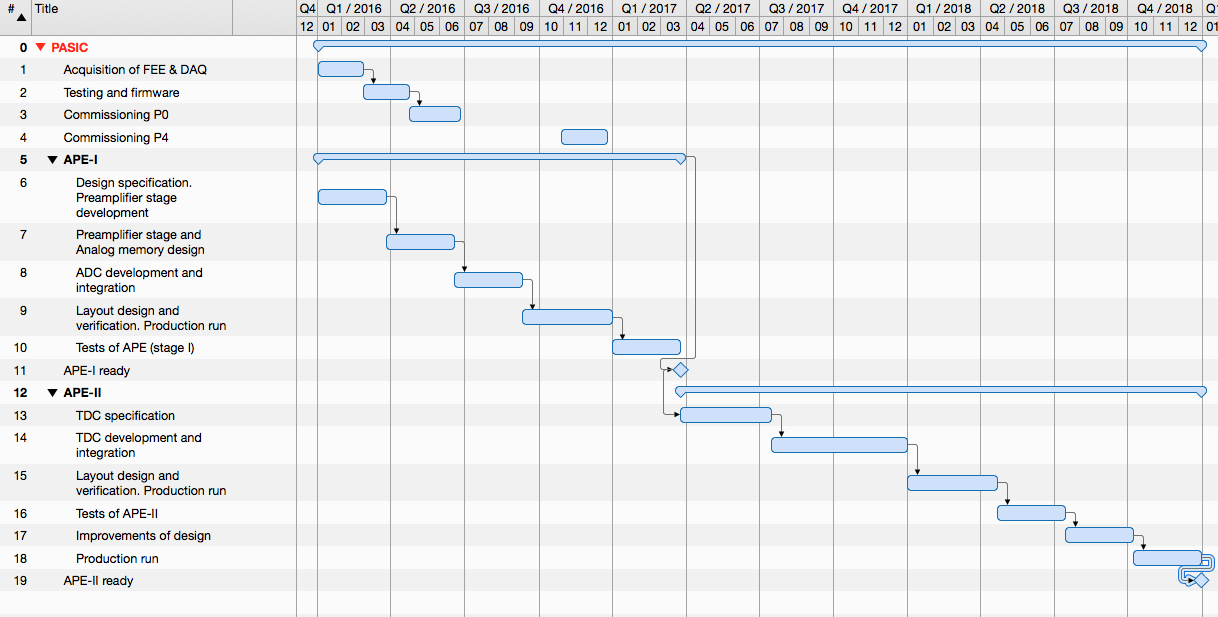
\includegraphics[scale=0.4]{img/ASICWF.png}
	\caption{\label{fig.ASICWF} Work flow of activities for ASIC.  }
\end{figure}

 
The design of APE will start early in the project, and will proceed in parallel with the development of P2 and P10. This will permit a first production run in 2016, and the possibility of testing the first stage in P2 during the first quarter of 2017. If the tests are successful P10 could then be equipped with the ASIC units rather than with discrete ADC cards. Specifically the lists of tasks and the development period is:

\begin{enumerate}
\item Design specification. Preamplifier stage development (Q1-16).
\item Analog memory design (Q2-16).
\item ADC development and integration. (Q3-16)
\item Layout design and verification. Production run (Q4-16)
\item Tests of APE in P4 (Q1/17)
\end{enumerate}
 
 The design of the full ASIC will then proceed during Q2/Q4-17, with the aim of a production run in Q1-18 and testing in P2 in Q2-18. If needed, a second run will occur in Q3-18, followed by testing in Q4-18. Figure \ref{fig.ASICWF} shows a flow diagram. 

\subsubsection*{Methodology of the IMG subproject}


\begin{figure}[!htb]
	\centering
	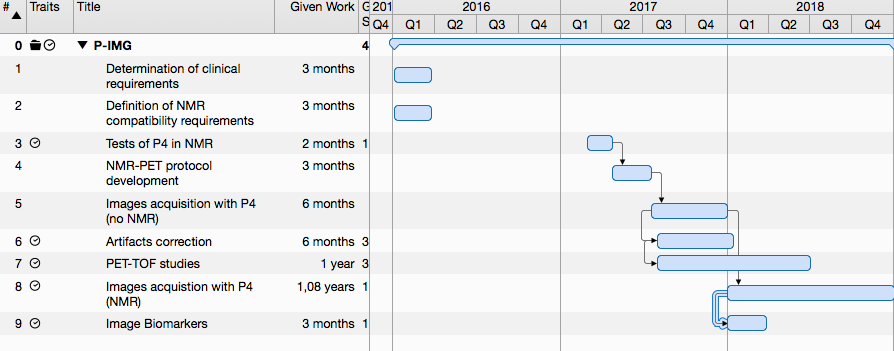
\includegraphics[scale=0.5]{img/ImgWF.png}
	\caption{\label{fig.ImgWF} Work flow for the activities of the IMG subproject.  }
\end{figure}

\paragraph{Definition of clinical requirements:}

In the very process of the PET device development some clinical requirement should be reached for an accurate spatial and temporal resolution. This requirements would be reviewed and studied from the existing literature and the state of the art.

Also, as the integration of both system will be performed in the La Fe Hospital installations, different compatibility prerequisite between PET and NMR will be evaluated to be considered in the PET development. Namely:
\begin{itemize}
\item The influence of the magnetic field on the new detectors developed. PETALO will be combined with a 3T (127Mhz) NMR device.
\item The size of the gantry of the NMR device, which is 60 cm.
\item The building materials of the PET device, which are meant to be adequate to avoid or have minimal artefacts in NMR images. 
\end{itemize}

\paragraph{NMR images acquisition}

In the final phase of prototype integration it will be necessary to test the compatibility of PETALO with the NMR system by performing several studies. These exams will comprise the development of protocols (sequences to be specified) for the acquisition of images with combined NMR and PET data and the storage of the images acquired into the hospital PACS

\paragraph{Integration of imaging biomarkers in the workflow}

The NMR-PET system will include the automated generation of imaging biomarkers derived from the acquisition profiles and sequences considered, like Pharmacokinetics imaging biomarkers extracted from MR Perfusion acquisitions (like vascular permeability, Ktrans; extraction rate, Kep; extra-vascular extra-cellular volume, ve) and also MR Diffusion (like apparent diffusion coefficient, ADC; and diffusion coefficient, D; pseudo-diffusion or perfusion coefficient, D*; vascular fraction, f). The automated quantification of the Metabolic Activity through the standardized uptake value (SUV) in the clusters with higher SUV values will be also developed\footnote{Ralf S. Eschbach , Wolfgang P. Fendler , Philipp M. Kazmierczak,, Marcus Hacker, Axel Rominger , Janette Carlsen , Heidrun Hirner-Eppeneder , Jessica Schuster , Matthias Moser , Lukas Havla , Moritz J. Schneider , Michael Ingrisch , Lukas Spaeth , Maximilian F. Reiser , Konstantin Nikolaou , Clemens C. Cyran Correlation of Perfusion MRI and 18F-FDG PET Imaging Biomarkers for Monitoring Regorafenib Therapy in Experimental Colon Carcinomas with Immunohistochemical Validation. PLoS One. 2015; 10(2): e0115543.}.

\paragraph{Testing the compatibility of P4 with NMR}
According to the schedule of the DET subproject, P4 will be built and characterised by Q4-16. In Q1-217 the detector will be installed inside the gantry of the NMR research apparatus available at the hospital La Fe (a 3T, 127Mhz apparatus with a 60 cm gantry). This is an essential test for the certification of PETALO as a fully compatible NMR apparatus. The compatibility requirements between NMR magnetic fields and P4 will be evaluated studying the influence of the magnetic field on the building materials, the sensors and ---as soon as available--- the (first stage) PETALO APE. The tests will run  through Q1-2017 and will include studies of combined PET and NMR data. 

\paragraph{Definition of clinical requirements and certification of P10}
During Q2-17, the quality and safety requirements to be used in a clinical environment will be defined, so that the system can be certified for operation at La Fe in Q2-17.

\paragraph{Study and modelling of image degradation phenomena for P10}

Like any PET device, PETALO will need a deep study to understand the  
degradation processes that affect the final determination of the images\footnote{Sune H. Keller,  Søren Holm, Adam E. Hansen, Bernhard Sattler, Flemming Andersen, Thomas L. Klausen, Liselotte Hojgaard,  Andreas Kjær, Thomas Beyer. Image artifacts from MR-based attenuation correction in clinical, whole-body PET/MRI. Magn Reson Mater Phy (2013) 26:173–181}. There are a number of them which will be of capital importance such as random coincidences, order of the sequence of the interactions, missing projection data, continuous energy spectrum of the gamma prompts, etc. These effects will be accurately modelled in order to minimise the negative impact in the imaging.

Most of these processes can be compensated at reconstruction time by computing a system matrix (SM) modelling the whole device. Other corrections can be added at hoc. However, the excellent timing and energy resolution expected for PETALO will likely a very well behaved SM. 

In summary, a dedicated image reconstruction software package for P4 will be developed. It should be flexible enough to accommodate many possible configurations. The device will be modelled with high degree of precision for achieving final images of the highest possible quality. 

According to the schedule P4 will be available in Q2-2017 for imaging studies after a full characterisation of its operational parameters (energy resolution, spatial resolution, CRT). The detector will then be operated for at least six months (Q3/Q4-17) as an imaging device (without magnetic fields) using phantoms and small animals to compute the SM and develop the imaging software.  

\paragraph{TOF imaging}

For image reconstruction, the Maximum Likelihood Estimation Maximization
(MLEM) is a commonly used method for PET and provides the possibility to include
Time-Of-Flight (TOF) information\footnote{Groiselle C J and Glick S J (2004): 3D PET list-mode iterative reconstruction using time-of-flight
information. IEEE Nucl. Sci. Symp. Conf. Record 2633-2638.}. The improvement in image quality achieved by TOF-MLEM reconstruction compared with standard MLEM for PET strongly depends
on the time resolution of the scanner. Currently, for commercially available crystal-based PET scanners the best coincidence resolving time (CRT) is currently   500-600 ps FWHM. As an example, the Philips Gemini TF made of LYSO and used for diagnostic PET shows 585 ps FWHM CRT\footnote{Surti S, Kuhn A, Werner M E, Perkins A E, Kolthammer J, and Karp J S (2007): Performance of
Philipps Gemini TF PET/CT Scanner with Special Consideration for Its Time-of-Flight Imaging
Capabilities. J Nucl Med 48 471-48}.
Recently, a new generation of PET scanners based on silicon photomultiplier provides
CRTs of 400 ps, as referenced in manufacturer data sheets (Philips Vereos PET/CT and
GE Signa PET/MR).

The IMG and the DET group will develop the TOF-MLEM reconstruction jointly to take advantage of the excellent CRT resolution expected for PETALO ($\sim 200-250$~ps), which would be, if confirmed, the best in the market. 

\paragraph{Acquisition of images with combined MR and PET data}
In 2018, P10 will operate inside the NMR gantry. 
The software for registration and fusion of the MR and PET images will be developed considering different techniques (segmentation, atlas-based) for the generation of attenuation maps in the PET images correction. Operation in the presence of magnetic field will run from Q1 to Q4 2018. The combination of the excellent energy and time resolution, TOF capabilities and NMR combined images should provide a strong demonstration of the strength of the technology. 

 

\subsubsection*{Infraestructuras, equipamientos y propuesta de co-financiaci\'on (equpamientos y fungible) / Infrastructures, equipment and co-funding request (equipment and fungible)}

%5. La descripción de los medios materiales, infraestructuras y equipamientos singulares a disposición de los participantes que permitan abordar la metodología propuesta.
\subsubsection*{Subproject DET}
\paragraph{Available Infrastructure and Equipment (IFIC)}

The PETALO group will work in close collaboration with the NEXT group, benefiting from the very well equipped laboratory (shared by both groups) which includes pressure and vacuum equipment, gas system, clean tent and an electronics workshop. Computing resources are also available at IFIC, as well as a good mechanical workshop. TPB coating facilities and bench stations for SiPM, and RGA and turbomolecular pumps are also amiable. 

\paragraph{Co-funding proposal}
Funding is requested for:

\begin{enumerate}
\item {\bf Fabrication of 4 LXSC2}, at a cost of 5,000 \euro per cell, adding up to 20,000 \euro
\item {\bf Fabrication of two small cryostats},  50,000 \euro.
\item {\bf Gas system for P4} (part of the gas system will be reused from de NEXT-DEMO detector,  20,000 \euro.
\item {\bf Vacuum, sealing and cryogenic parts}, for an approximate cost of 10,000 \euro.
\end{enumerate}

The equipment requested adds up to 100,000 \euro.  
Te adjunto el parrafito sobre infraestructura relativo al grupo I3M-UPV. 

\paragraph{Available Infrastructure and Equipment (I3M-UPV)}
The I3M-UPV research team has full access through Europractice to professional ASIC design tools. Cadence Design Systems tool framework has been chosen for mixed signal microelectronics developments due to its compatibility with most of the available design kits provided by silicon foundries. It integrates both digital and analog design flows from high abstraction level descriptions (HDL code) to schematics design entry (preferred in Analog designs) and final layout integration. Along with design tools, Cadence offers high-end simulation (Spectre, AMS), physical processing and verification (ASSURA) tools. Thus the whole design flow can be covered inside the same environment using the simulation and parasitics extraction models included in the selected technology process design kit. The mandatory non-disclosure agreements (NDA) have already been signed in order to obtain access to Austria MicroSystems Foundry Services for 0.35 um and 0.18 um processes. Those are one of the most common technologies being used nowadays for the kind of ASICs being proposed in this project.

\par High performance computing hardware is available to develop the design, simulation and verification tasks associated to microelectronics developments:
\begin{itemize}
 \item 2 Fujitsu RX200S8 (64 GB de RAM, Xeon E52660V2 x2) workstations in a rack installation inside I3M computing center.
 \item 1 Fujitsu Eternus Disk Vault acting as centralized disk space server (6 TB / RAID 5).
\end{itemize}

\par I3M-UPV group can also contribute with electronics laboratory equipment in order to build a test bench for test and characterization of the sample prototypes delivered by the silicon foundry:
\begin{itemize}
 \item Keithley 2230-30-1 Programmable Low noise Power Supply with 3 individual outputs.
 \item Lecroy WaveSurfer 104MXs-B (10GS/s) 4 channel oscilloscope for high bandwidth measurements
 \item 4 LXI ZTEC Oscilloscopes (150 MHz / 16 Channels) for general test and characterization
 \item Fluke Ti125 9Hz Thermographic Camera for thermal reliability measurements.
 \item SMD soldering facilities with high resolution camera display for prototype PCB handling.
\end{itemize}

\paragraph{Co-funding Request}
\par There two requests of funding related to I3M-UPV group activities in the project:
\begin{itemize}
\item First of all the computing hardware should be improved in order to be able to simulate the ASIC in the final stage of development. We foresee that the proposed integrated front-end will need of more computing power for verification and sign-off simulations. The cost of another two similar workstations is 6,100 €
\item The annual fees due to Europractice membership maintenance which are needed to obtain the research degree software licenses. The cost of the Cadence design framework is 2,150 € and a special fee of 1,100 € has to be fulfilled in order to access foundry services.
\end{itemize}

\par The total cost of extra infrastructure and fungible needed for the project will be 9,350 €
\subsubsection*{Subproject IMG}
\paragraph{Available Infrastructure and Equipment (GIBI230-LaFe)}

The research group GIBI230 is located and develops most of its work at the University and Polytechnic hospital La Fe, referral hospital in the Valencia community and one of the major hospitals in the Spanish territory, and especially at the Medical Imaging Clinical Area. 
This Medical Imaging Clinical Area has in one hand a Radiology Section with several CT devices (TC Brillance 64 Philips (2 devices), TC Brillance iCT 256 Philips, TC O-arm
Medtronic, TC Aquilion 64 Toshiba), densitometers (Discovery DXA Hologic) and X-RAY devices (Philips Digital Diagnost). On the other hand, in the Nuclear Medicine Section are available 3 SPECT/CT (Philips Brightview XCT) and a PET-CT device (Philips Gemini TF 64 with “TrueFlight” technology) the only PET/CT device in the public system of the Valencian Community.

Also the Medical Imaging Clinical Area (GIBI 230) boasts of Experimental Radiology Unit in which this project will be developed with a specific area of animals preparation annexed to the animal facility of the Institute for Health Research La Fe.

This space has a MRI device of 3T from Philips (Achieva 3.0T TX) specific to research. Jointly there is also a workstation for image processing Imalytics model (only 60 in the world), product of Philips Healthcare for their reference research centers. For the projects of the group there is also space in the hospital PACS dedicated to research, in which free space will be allocated by AGFA for storing images, thanks to a Master Research Agreement between this company and the hospital for the development of innovative projects in medical imaging.

\paragraph{Co-funding proposal}
 This project only requires co-funding for the tests of compatibility (use of the NMR apparatus). estimated in 18,000 \euro. 


\subsubsection*{Cronograma / Timetable}


\begin{figure}[!htb]
	\centering
	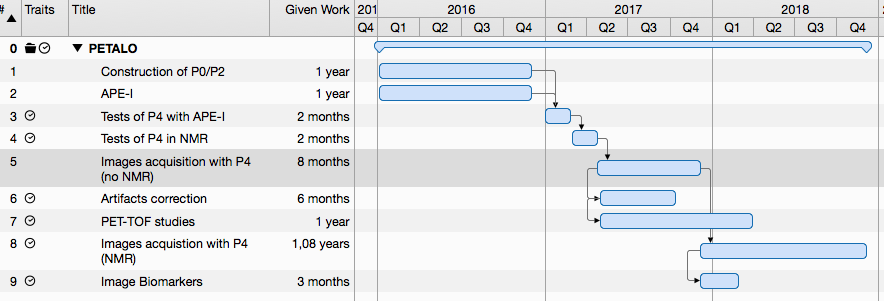
\includegraphics[scale=0.5]{img/Crono.png}
	\caption{\label{fig.Crono} Cronogram of the PETALO project.  }
\end{figure}

The work flow of the different projects has been detailed in the Methodology. Figure \ref{fig.Crono} shows a simplified cronogram to illustrate the development of the project.
%\input{src2/BataSchedule.tex}

\subsubsection*{Personal / Personnel}

%7. Si se solicita ayuda para la contratación de personal, justificación de su necesidad y descripción de las tareas que vaya a desarrollar.
\paragraph{Personnel resources and requirements of the DET subproject:}

The feasibility of the DET subproject is based in the availability at IFIC of three engineers who have worked during the past five years in the NEXT experiment and have acquired the expertise and know-how needed to make feasible the construction of P2 and P10. Specifically we refer to J. Rodriguez and V. Álvarez, both of them leading electronics engineers working in the NEXT tracking plane and to Alberto Martínez, a mechanical engineer who has been the leading mechanical designer for NEXT.
These engineers have been payed up to know with funds associated to the NEXT project with exclusive dedication to NEXT. Indeed, their dedication to NEXT will be 100\% until the end of 2015, but the work load of the electronics and mechanics engineers in NEXT will be smaller than usual in 2016, and their time can be shared with the PETALO project. Furthermore, these engineers have obtained 3-year contracts as ``support technicians" (técnicos de apoyo) to work at IFIC. They will start their contracts in later 2015 or early 2016, at which point they will no longer be payed by NEXT. 
Moreover there is a Ph. Student, Francisco cortés who is starting a Ph. D. Thesis on simulations of the Petalo Detector, and a technician,  Vanesa Delgado who has experience in cryogeny, and has worked during years with germanium detectors. 
J. Rodriguez and V. Álvarez will collaborate in the construction of the liquid xenon cells, and  V. Delgado and A. Martínez  will participate in the design and construction of the cryostat.

In summary, the timing of this project is ideal for the optimal utilisation of the engineering resources available at IFIC which would make it possible a smooth technology transfer from NEXT to PETALO. 


In addition to the engineers mentioned above, and the PI (who will be fully dedicated to PETALO) the DET project requires two full-time doctors. The first doctor, with an instrumental profile (Post-doc DET), will work in the construction, commissioning and operation of P2 and P10 and will supervise and be responsible with the PI   all the tasks of construction of cells, cryostat and gas system. He or she will benefit from the expertise developed at IFIC during the operation of the DEMO detector from 2011 to 2015, as well as from the existing infrastructures, which include a fully operative xenon gas depuration system, which will be reused by P0 and P4. This 

 The second post-doc will be leading the development of SIMPLE and RAP as well as the characterisation of P0 and P4 at IFIC. She will also contribute to the imaging software analysis, in particular concerning the PET-TOF application of the device, in collaboration with francisco Ortega.
 
This project requires funding for a post-doc during three years. We are confident that additional personnel resources can be obtained by presenting suitable candidates to he ``young investigators'' MINECO program as well as to other funding bodies (IFIC Severo Ochoa program, Juan de la Cierva, etc). In particular,  
Dr. Paola Ferrario, who has played a leading role in the development of the NEXT software during the last three years and would be the perfect candidate for the software post-doc will apply to these programs. 
 
 \paragraph{Personnel resources and requirements of the ASIC subproject:} 

The ASIC subproject is based in the expertise existing  at the I3M/UPV, which includes the to co-PIs, Prof. V. Herrero Bosch (VHB), Prof. Rafael Gadea (RG) on one side and professors J. F. Toledo (JFT) and R. Esteve (RE) on the other. VHB and RG are leading developers of ASIC for PET and their extensive experience qualifies them uniquely for developing a new ASIC for PETALO. On the other hand, JFT and RE have been the leading developers of the FEE and DAQ for the NEXT experiment. The solutions that PETALO has adopted for the initial operation of P2 and P10 are based in the solutions tried and tested by NEXT, as described previously. 
In addition the group has two students currently working with VHB.

The project requires an electronic engineer (Eng ASIC), who will be in charge of the daily tasks related with the acquisition, assembly and testing of the ATCA electronics used during the initial run of P2 and P10.  He or she will also develop the slow control system. The engineer will be closely supervised by JFT and RE, who have extensive experience but can devote only a fraction of their time to this project. The development of the ASIC will be entirely the responsibility of VHB, RG and their students. 

 \paragraph{Personnel resources and requirements of the IMG subproject:}
 The IMG subproject includes an interdisciplinary team, lead by Dr. Irene Torres, a nuclear physicist with a Ph.D. in medical imaging. 
 
 The project requires a post-doc who whose activities will be in the area of imaging requirements, reconstruction and integration of image post-processing and the extraction of imaging biomarkers.
 
The post-doc background will be focused in the field of biomedical engineering and medical physics, specially in medical imaging acquisition technologies (PET and NMR systems) and in medical imaging processing.
 
The tasks to be addressed by the Post-Doc will be under the frame of the integration of the PET solution with the NMR, the requirements of the new technology and the aspects of image reconstruction and processing. These will include:
 \begin{enumerate}
\item Definition of MRI compatibility requirements and clinical spatial resolution.
\item Study and modelling of image degradation phenomena LXSC-PET.
\item Mathematical modelling of signals from PET detectors.
\item Integration in the software of the user interface of the system.
\item Development of hybrid image reconstruction methods for PET-MRI.
\item Development of algorithms for the extraction of imaging biomarkers.
\item Integration of imaging biomarkers analysis in user interface.
\end{enumerate}


\vspace{12pt}

\noindent\textbf{C.3. IMPACTO ESPERADO DE LOS RESULTADOS / EXPECTED IMPACT}

%C.3. IMPACTO ESPERADO DE LOS RESULTADOS 

The expected impact of this project is very large. A successful proof of concept of PETALO would open the way to the subsequent construction of pre-clinical (e.g, small animal PET) and clinical PETs. PETALO offers many advantages over conventional SSDs based devices, including a much better energy resolution, true 3D reconstruction that minimises parallax effects and the capability to handle Compton interactions, which are much better identified in the LXSC than in conventional SSDs. In addition, PETALO will be designed, from the beginning, as a fully compatible device with NMR, including both hardware components and the development of the imaging software. On top of the above, PETALO offers the potential of a breakthrough in TOF-PET technology. Last, but not least, the cost of the detection material (LXe) is much lower than the cost SSDs such as LSO and the cost of the SiPMs is decreasing exponentially. Therefore, by developing suitable front-end electronics and DAQ, PETALO could become a very economical PET solution, appropriated for a future large-scale (full-body) PET.

Each subproject in this coordinated project contributes in a decisive way to the impact of PETALO. Subproject DET focuses in transferring the technology developed by a basic science experiment (NEXT) to an application of enormous importance for public health. Subproject ASIC is essential, not only to provide the needed electronics for the proof of concept, but to develop the APE chip, which is mandatory for a large-scale application. The subproject IMG will, from the very beginning, focus in the integration of PETALO and NMR. 

PETALO has already produced a patent request, and a number of other patents will certainly follow. The apparatus can be clearly commercialised, given its many advantages over conventional PETs. The diffusion of the results will proceed through publications in journals and participation in national and international conferences. Once the proof of concept is operational, the research team will work actively with companies to explore join ventures and possibilities of transferring to the industrial sector. 


\vspace{12pt}

\noindent\textbf{C.4. CAPACIDAD FORMATIVA DEL EQUIPO / TRAINING CAPABILITIES OF THE GROUP}
The PETALO project represents a unique opportunity for training students. 

\subsubsection*{Training Capabilities of the IFIC group}

The PI of the project has supervised more than 10 Ph.D. thesis during his career. The student will have the unique opportunity to work in the construction of P0 and P4, commission and analysis the data produced by the apparatus, and later participate in the imaging analysis, in particular concerning the TOF capabilities. The development of the thesis would correspond to the tasks described in the plan presented for DET. In particular, the plan of studies will include:

\begin{enumerate}
\item {\bf Study of the energy resolution using photoelectric events.} Photoelectric events are easily characterised in the LXSC, as single-site deposition events (unless conventional SSDs, the LXSC can separate multiple-site events to an expected resolution of a few mm). Then, the energy in the LXSC is measured by adding the signal of all the SiPMs. The energy resolution is obtained by fitting the photoelectric peak. The energy resolution of the LXSC6 will be measured as reference (an energy resolution of better than 3\% FWHM is expected). Then, the energy resolution of the LXSC2 will be measured. A resolution better than 5\% FWHM is expected.
\item {\bf Study of the position resolution using photoelectric events.} To estimate the position resolution from data, we will use the LXSC6 which provides 2 redundant measurements of each coordinate. Then, if $\chi_1,\chi_2$~are redundant measurements of a given coordinate, and $\Delta \chi = \chi_2 - \chi_1$~is the difference between them, the $\Delta \chi$ distribution should have mean zero and standard deviation  
$\delta \Delta \chi \sim \sqrt{2} \delta \chi$. To estimate the position resolution of LXSC2, one starts by validating the Monte Carlo simulation of the LXSC, by comparing data and Monte Carlo results for the LXSC6. After demonstrating that the Monte Carlo reproduces correctly the simulation measured with data for the LXSC6, one can use the Monte Carlo to estimate the position resolution of LXSC2. Position resolution in the range of 1-2 mm are expected. 
\item {\bf Study of the time resolution using photoelectric events.} Coincidence Resolution Time (CRT) will be measured by comparing the time stamp provided by the two opposite LXSC cells. A CRT in the range of 200-250 ps is expected.
\end{enumerate}

In addition, a program of studies for Compton interactions (starting with Compton events that deposit their full energy in the cell and show a double-site deposition, will be carried out. The program will include the study of the energy, position and time resolution for double-site Compton events, the study of the resolution to separate double-site events, and the feasibility of using Compton kinematics to improve the resolution of the back projected tracks. 


\subsubsection*{Training Capabilities of the I3M-UPV group}
\par The research team has already directed 5 Doctoral Thesis and is being directing 2 more at the moment. Both members of the research team have long experience in graduate and post-graduate teaching since they work as Associate Professors in the Electronics Engineering Department of "Universitat Politècnica de València". The PETALO project may become a source for Doctoral Thesis proposal which could serve as evaluation of alternative solutions for the front-end architecture. For instance a further reduction of the DAQ deadtime would be desirable in order to increase maximum event rate. The proposed solution in PETALO would increase ASIC complexity to an unaffordable level if deadtimes under 0.5 $\mu$s must be achieved. However a scheme based on deep analog FIFOs may lead to better solutions yet many issues related to noise, signal degradation etc should be first solved.
\par A usual work plan for a Doctoral Thesis in microelectronics for front-end integration should cover a three years time span as follows:
\begin{description}
  \item[TASK 1 (6 Months)] Complementary training and State of the Art review. Depending on the proposal some specific training might be needed by the student. A mandatory review of the state of the art will help to focus on the problem.
  \item[TASK 2 (2 Month)] Design Specifications. Selection of technology node and design tools.
  \item[TASK 3 (3 Months)] High level modeling of analog and digital blocks. A set of high level modelling languages will be used in order to obtain functional detailed models of the different blocks.
  \item[TASK 4 (4 Months)] Architectural Simulations based on previous models to determine design trade-offs
  \item[TASK 5 (5 Months)] Analog design. All the analog blocks will be designed and validated in a multilevel simulation testbench using digital block models.
  \item[TASK 6 (3 Months)] Digital design.
  \item[TASK 7 (4 Months)] Layout design, Parasitics Extraction and Simulation. The effects of parasitics due to layout design are included in simulations and the whole system can be simulated as a final verification process before production.
  \item[TASK 8 (1 Month)] Sign-off preparation and Foundry first iteration (Cross design rule check, bonding diagram and package selection)
  \item[TASK 9 (4 Months)] Prototype test and characterization. A testbench (including a PCB carrier) must be designed in order to test the prototype. A test protocol must be defined and a final characterization data sheet produced.
  \item[TASK 10 (4 Months)] Thesis writing and results publishing. Some of the preliminary results (especially those related to the analog design) can be published before depending on their scientific value.
\end{description}

\subsubsection*{Training Capabilities of the GIBI230 group}
The Principal Investigator and the members of the research group form a multidisciplinary team including physicists, nuclear physicians and telecommunications engineers inside the Biomedical Imaging Research Group GIBI230. This research group has huge experience in the training of fellows belonging to several universities from the Spanish territory and also from abroad directing thus BSc’s and MSc’s thesis as PhD thesis. Furthermore, the members of the research team have participated as teachers in several courses and seminars related to the project topic. 
The research team members have experience in training students of different backgrounds, such as Physics or Medicine and also Biomedical Engineering, being two of the members, former trainees of their Biomedical Engineering master’s thesis.
The research team and the training fellow will have enough resources and equipment available to properly develop the assigned task of the project in the Medical Imaging Clinical Area of the University and Polytechnic Hospital La Fe. 
This experience indicates that the research team has sufficient training capacity to assume the incorporation of training fellow who could finish the doctoral thesis within the period of the project. 


%Este apartado solo se rellenará si alguno de los subproyectos participantes solicita la inclusión del proyecto en la convocatoria de “Contratos predoctorales para la formación de doctores”. Dicha inclusión solo será posible en un número limitado de los proyectos aprobados.
%
%Para evaluar la capacidad formativa del equipo solicitante, se recomienda incluir:
%
%1. El plan de formación previsto.
%
%2. Relación de tesis realizadas o en curso (últimos 10 años) con indicación del subproyecto, nombre del doctorando, el título de tesis y la fecha de obtención del grado de doctor o de la fecha prevista de lectura de tesis.
%
%3. Breve descripción del desarrollo científico o profesional de los doctores egresados de los equipos de investigación de los subproyectos participantes.

%%%%%%%%%%%%%%%%%%%%%%%%%%%%%%%%%%%%%%%%%%%%%%%%%%%%%%%%%%%%%%%%%%%%%%%%%%%%%

\vspace{12pt}

\noindent\textbf{C.5. IMPLICACIONES ÉTICAS Y/O DE BIOSEGURIDAD/ETHICS AND SAFETY IMPLICATIONS}

This project focuses in a proof of concept that will operate mostly with phantoms and eventually with small animals, under the control and regulations operative at the hospital La Fe. Thus there are no ethical or safety implications to take into account. 


\end{document}

